\documentclass[letterpaper]{ar-1col}
\usepackage{showyourwork}
\usepackage[letterpaper]{geometry}

\usepackage{natbib}
\usepackage{amsmath}
\usepackage{color}
\usepackage{hyperref}
\usepackage{mhchem}
\usepackage{booktabs}% http://ctan.org/pkg/booktabs
\newcommand{\tabitem}{~~\llap{\textbullet}~~}
\hypersetup{colorlinks=true,allcolors=[rgb]{0,0,0.8}}

\newcommand{\kms}{km~s$^{-1}$}
\newcommand{\mum}{$\mu$m}
\newcommand{\ld}{$\lambda/D$}
\newcommand{\fourier}[1]{\mathcal{F}\{#1\}}
\newcommand{\invfourier}[1]{\mathcal{F}^{-1}\{#1\}}
\newcommand{\acc}[1]{\entry{\acs{#1}}{\acl{#1}}}

\usepackage{multicol}%for multiple columns
\usepackage{etoolbox}

\usepackage{nomencl}
\makenomenclature
\setlength{\nomitemsep}{6pt}

% multiple columns for nomencl
% https://latex.org/forum/viewtopic.php?t=14564
 \renewcommand*{\nompreamble}{\begin{multicols}{2}}
\renewcommand*{\nompostamble}{\end{multicols}}
\setlength{\columnsep}{3em}

\usepackage{graphbox}

\setcounter{secnumdepth}{4}
\usepackage{url}


% https://tex.stackexchange.com/questions/163451/total-number-of-citations
\usepackage{totcount}
\usepackage[nolist,nohyperlinks]{acronym}

\begin{acronym}
\acro{aplc}[APLC] {Apodized Phase Lyot Coronagraph}
\acro{paplc}[PAPLC] {Phase Apodized Phase Lyot Coronagraph}
    \acro  {psf}[PSF]   {Point Spread Function}
    \acro  {iwa}[IWA]   {Inner Working Angle}
    \acro  {owa}[OWA]   {Outer Working Angle}
    \acro  {ao}[AO]     {Adaptive Optics}
    \acro  {fpm}[FPM]   {Focal Plane Mask}
    \acro  {ppm}[PPM]   {Pupil Plane Mask}
    \acro  {hz}[HZ]     {Habitable Zone}
    \acro {fpwfs}[FPWFS]{Focal Plane Wavefront Sensing}
    \acro  {fwhm}[FWHM] {Full Width Half Maximum}
    \acro  {fqpm}[FQPM] {Four Quadrant Phase Mask}
    \acro  {agpm}[AGPM] {Annular Groove Phase Mask}
    \acro  {ovc}[OVC]   {Optical Vortex Coronagraph}
    \acro  {pp}[PP]     {Pupil Plane}
    \acro  {fp}[FP]     {Focal Plane}
    \acro  {hci}[HCI]   {High Contrast Imaging}
    \acro  {dm}[DM]     {Deformable Mirror}
    \acro  {wfs}[WFS]   {Wavefront Sensor}
    \acro  {zwfs}[ZWFS] {Zernike Wavefront Sensor}
    \acro  {sphere}[SPHERE]{Spectro-Polarimetric High-contrast Exoplanet REsearch}
    \acro  {scfp}[SCFP] {Science Camera Focal Plane}
    \acro  {smd}[SMD]   {Spatial Mode Demultiplexing}
    \acro  {ncpa}[NCPA] {Non-Common Path Aberration}
    \acro  {mspl}[MSPL] {Mode-selective Photonic Lantern}
    \acro  {elt}[ELT]   {Extremely Large Telescope}
    \acro  {jwst}[JWST] {James Webb Space Telescope}
    \acro  {gmt}[GMT]   {Giant Magellan Telescope}
    \acro  {tmt}[TMT]   {Thirty Metre Telescope}
    \acro  {sp}[SP]     {Shaped Pupil}
    \acro  {scc}[SCC]   {Self Coherent Camera}
    \acro  {fast}[FAST] {Fast Atmospheric SCC}
    \acro  {smscc}[SM-SCC] {Spectrally Modulated SCC}
    \acro  {app}[APP]   {Apodizing Phase Plate}
    \acro  {gvapp}[gvAPP]   {grating vector Apodizing Phase Plate}
    \acro  {vvc}[VVC]   {Vector Vortex Coronagraph}
   \acro  {vfn}[VFN]    {Vortex Fibre Nulling}
   \acro  {ravc}[RAVC]  {Ring Apodized Vortex Coronagraph}
    \acro  {hwo}[HWO]   {Habitable Worlds Observatory}
%% Define a custom plural form of an acronym   
    \acrodefplural{psf}[PSFs]   {Point Spread Functions}
    \acrodefplural{dm}[DMs]     {Deformable Mirrors}
    \acrodefplural{wfs}[WFSs]   {Wavefront Sensors}
    \acrodefplural{elt}[ELTs]   {Extremely Large Telescopes}
    \acrodefplural{ncpa}[NCPAs] {Non-Common Path Aberrations}
%% Preferably, put all acronym definitions in one file and load it
%   \input{acros.tex}
\end{acronym}

\newtotcounter{citnum} %From the package documentation
\def\oldbibitem{} \let\oldbibitem=\bibitem
\def\bibitem{\stepcounter{citnum}\oldbibitem}
%%%%

\usepackage{lipsum}  

% Metadata Information
\jname{Annu. Rev. Astron. Astrophys.}
\jvol{AA}
\jyear{2025}
\doi{10.1146/TBD}

% autoref formatting
\def\sectionautorefname{Section}
\let\subsectionautorefname\sectionautorefname
\let\subsubsectionautorefname\sectionautorefname

% macros
\newcommand{\apjl}{Astrophysical Journal Letters}
\newcommand{\aj}{Astronomical Journal}
\newcommand{\ao}{Applied Optics}
\newcommand{\procspie}{SPIE Proceedings}
\newcommand{\apj}{Astrophysical Journal}
\newcommand{\apjs}{Astrophysical Journal Supplement}
\newcommand{\pasp}{Publications of the Astronomical Society of the Pacific}
\newcommand{\jgr}{Journal of Geophysical Research}
\newcommand{\aap}{Astronomy and Astrophysics}
\newcommand{\aapr}{Astronomy and Astrophysics Review}
\newcommand{\mnras}{Monthly Notices of the Royal Astronomical Society}
\newcommand{\actaa}{Acta Astronomica}
\newcommand{\nat}{Nature}
\newcommand{\prl}{Physical Review Letters}
\newcommand{\prd}{Physical Review D}
\newcommand{\ssr}{Space Science Reviews}
\newcommand{\araa}{Annual Review of Astronomy and Astrophysics}
\newcommand{\jrasc}{Journal of the Royal Astronomical Society of Canada}
% Symbols
\newcommand{\ydata}{\ensuremath{\boldsymbol{y}}}
\newcommand{\hyperparams}{\ensuremath{\boldsymbol{\phi}}}
\newcommand{\meanparams}{\ensuremath{\boldsymbol{\theta}}}
\newcommand{\dt}{\ensuremath{\tau}}
\newcommand{\amplitude}{\ensuremath{\alpha}}
\newcommand{\lengthscale}{\ensuremath{\lambda}}

\DeclareMathOperator*{\argmax}{arg\,max}

\newcommand{\project}[1]{\textsf{#1}}

% Comments:
\newcommand{\commentmak}[1]{\textcolor{red}{[MAK: #1]}}
\newcommand{\commentsyh}[1]{\textcolor{red}{[SYH: #1]}}

\newcommand{\notebooksuggestion}[1]{\textcolor{blue}{[Notebook: #1]}}

\newcommand{\todo}[1]{\textcolor{red}{[TODO: #1]}}

% message://%3cBYAPR04MB46634305E3091DE92934A5BA8225A@BYAPR04MB4663.namprd04.prod.outlook.com%3e

% Manuscript due date:  September 15, 2024
% Article allotment: 18,000 words, 200 references

% message://%3cCB3B5076-708A-441A-B38E-4050212CB3EA@strw.leidenuniv.nl%3e
% message:/%3cBYAPR04MB466383143958CB8F10DE8D8E82112@BYAPR04MB4663.namprd04.prod.outlook.com%3e

% about 14,400 words, with 11 figures, 40 pages

% (Estimate the sizes of small figures/tables at 300 words and large ones at 600 words; thus, for every figure/table submitted, please subtract the corresponding number of words from your total allotment. An article length estimator is available online at http://www.annualreviews.org/page/authors/general-information; to access it, select the name of your journal from the drop-down list under Article Preparation and Submission.)  

% Your review article should present a critical appraisal of the significant, rather than the total, literature in the field. This overview may include your own work (even if unpublished). The article should be useful to specialists as well as teachers and scholars from other areas.  It should emphasize where research in a given area should go, as well as where it has been, such that it will influence the future course of knowledge. A list of topics and authors planned for Volume 63 will be sent to you approximately five months before the manuscript due date, and you may wish to correspond with authors whose subjects border on your own.

% Document starts
\begin{document}

% Page header
\markboth{Kenworthy \& Haffert}{HCI}

%TC:ignore

% Title
\title{High Contrast Coronagraphy}

%Authors, affiliations address.
\author{Matthew Kenworthy$^1$ and Sebastiaan Haffert$^{1,2}$
  \affil{$^1$Leiden Observatory, Niels Bohrweg 2, Leiden 2300RA, The Netherlands; email: kenworthy@strw.leidenuniv.nl}
  \affil{$^2$Steward Observatory; email: haffert@strw.leidenuniv.nl}}


% Abstracts should include 3–5 bullet points citing actual conclusions of the review. Please limit the abstract to no more than 200 words, including the bullet points. If using TeX, use a “\hangindent=.3cm$bullet$” command at the beginning of each bullet-point paragraph. [The “\begin{itemize}” environment may require the use of a “hardwired” line return (i.e., the ”\\” command) within the environment, as lines may not automatically return in the compiled version.]
%Abstract
\begin{abstract}
Imaging terrestrial exoplanets around nearby stars is a formidable technical challenge, requiring the development of coronagraphs to suppress the stellar halo of diffracted light at the location of the planet.
%
In this Review, we derive the science requirement for high contrast imaging, give an overview of diffraction theory and the Lyot coronagraph, and define the parameters used in our optimization.
%
We detail the working principles of coronagraphs both in laboratory and on-sky with current high contrast instruments, and detail the required algorithms and processes necessary for terrestrial planet imaging with the extremely large telescopes and proposed space telescope missions.

\begin{itemize}
    \item Imaging terrestrial planets around nearby stars is possible with \\ 
    a combination of coronagraphs and active wavefront control \\
    using feedback from \acp{wfs}.
    \item Ground based 8-40m class telescopes can target the habitable \\ 
    zone around nearby M dwarf stars with contrasts of $10^{-7}$ and \\
    space telescopes can search around solar-type stars with \\
    contrasts of $10^{-10}$.
    \item Focal plane wavefront sensing, hybrid coronagraph designs and \\
    multiple closed loops providing active correction are required \\
    to reach the highest sensitivities.
    \item Polarization effects need to be mitigated for reaching $10^{-10}$ \\ contrasts whilst keeping exoplanet yields as high as possible.
%    \item Ground based telescopes require fast ($\ge$ 1kHz) closed loop \\
%    adaptive optic systems and high density deformable mirrors to \\
%%    minimise the wind-driven halo seen in the science camera focal \\
 %   plane.
    \item Recent technology development, including photonics, MKIDS \\
    and QOD will be folded into HC instruments.
\end{itemize}

\end{abstract}

%Keywords, etc.
\begin{keywords}
 Optics, coronagraphs, exoplanets, high contrast, computational methods
\end{keywords}
\maketitle

%Table of Contents
\tableofcontents

\section{INTRODUCTION}
\label{sec:intro}

% High contrast imaging, Lyot corongraph, 2000's development

%TC:endignore

%In this review, we provide interactive notebooks that enable the reader to build up their intuition on how coronagraphs work along with wavefront sensing both in the pupil and the focal planes, and how we will tackle the challenges in reaching the contrasts of $10^{-10}$ at angular separations of less than one arcsecond that are required.

% text below from DFM

%To see the specific version of the \project{Jupyter} notebook, that was executed to generate each figure, click on the icon next to the figure caption.

Initially developed to image the Sun's corona without the need for a Solar eclipse \citep{Lyot33}, one of the most significant science drivers for the latest coronagraphs is in the detection and characterisation of circumstellar material and planets around nearby stars.
%
Young self-luminous gas giant exoplanets have been discovered around young stars \citep[see ][ for a review of these detections]{Zurlo24} both in the nearby Galactic field (HR8799b,c,d, Beta Pic b and c) and further away in young stellar OB associations ranging from 80 to 200 pc distance, typically these exoplanets have luminosities of $10^{-4}-10^{-6}$ at angular separations of up to one or two arcseconds from their parent star. 

\begin{armarginnote}[]
  \acc{hci}
  \acc{fp}
  \acc{pp}
  \acc{fpwfs}
  \acc{wfs}
\end{armarginnote}

At optical wavelengths, exoplanets are not self-luminous but instead reflect the light of their parent star.
%
For an Earth analogue with similar radius, albedo and effective temperature orbiting around a solar-type star 10 parsecs away, the typical amount of reflected light in the optical is $10^{-10}$ of the central star at a separation of 0.1 arcseconds at maximum elongation.
%
The technical challenge is in distinguishing the light of the parent star from the light of the planet.
%
Planetary systems that are closer to the Sun have two benefits: one that is twice as close as the other will have double the angular separation between the star and planet, and from the inverse square law, four times more flux is received from the planet.
%
For direct imaging, therefore, the closest stars to the Sun are the ones that are studied for the presence of directly imaged exoplanets.
%
On average there are more M dwarf stars close to the Sun than other solar type stars: in a volume limited (20 parsec) sample around the Sun, there are $\sim 140$ solar G-type stars, and on the order of 1900 M-dwarf stars \citep{Kirkpatrick24}.
%
For solar type stars, the contrast required in the optical wavelengths is on the order of $10^{-10}$ for terrestrial planets in the HZ of solar type stars, but for smaller mass stars with lower luminosities, the contrast is $10^{-7}$ for M dwarfs.



%Using Fresnel zones to make a circular null around the star \citep{Angel86} first time you could detect a Jupiter around a sun-like star.

\begin{figure}[ht]
  \centering
%  \script{plot_flux_ratio.py}
  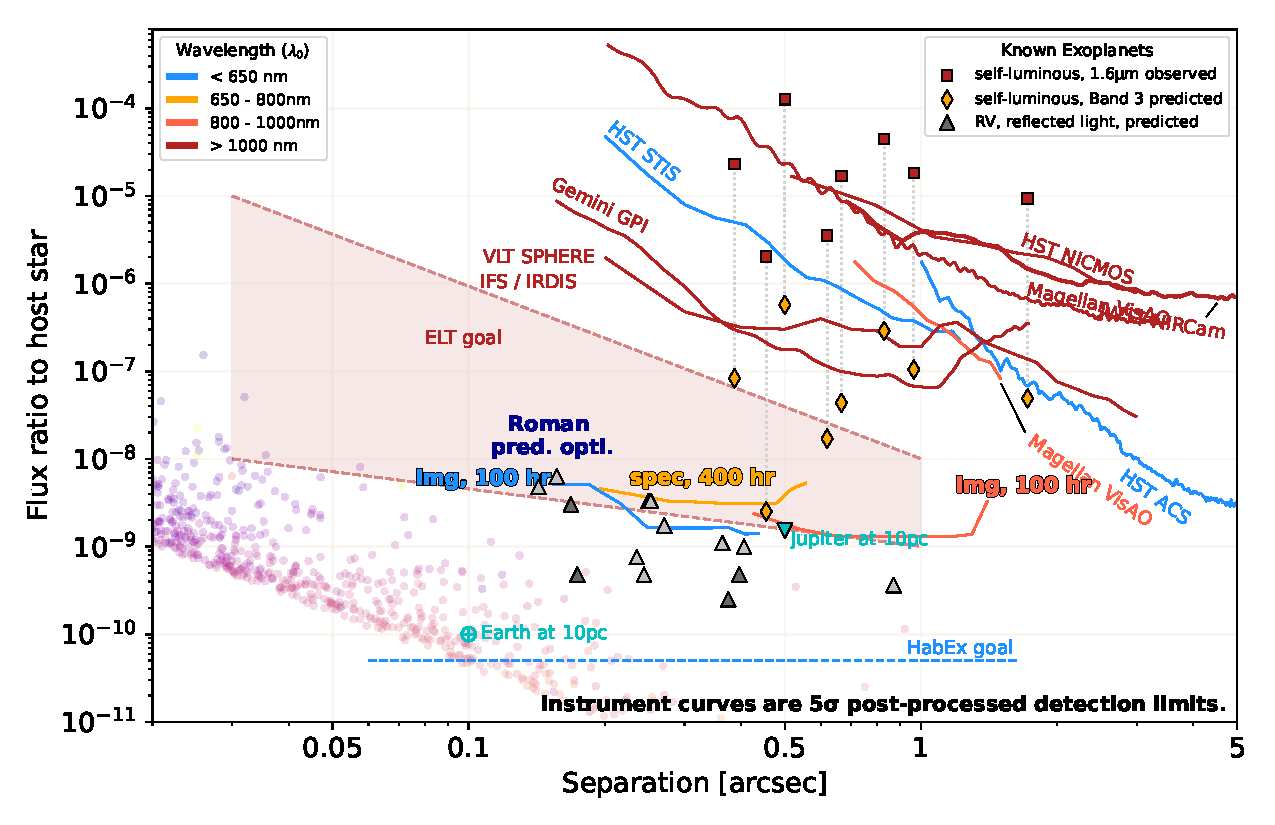
\includegraphics[width=1.0\linewidth]{figures/flux_ratio_default_opti.pdf}
  \caption{Figure plot and data from \citet{Bailey24} \href{https://github.com/nasavbailey/DI-flux-ratio-plot}{Bailey and Rafels(2024)  {\tt github.com/nasavbailey/DI-flux-ratio-plot}}. Reflected light estimates for 1 Earth radius planets, assuming one planet per star within 20 parsecs of the Sun in the Habitable Zone at maximum elongation (data from \href{https://subarutelescope.org/staff/guyon/04research.web/14hzplanetsELTs.web/catalog.web/content.html}{Guyon 2024 web page}).  Lines and points are color coded by wavelength of observation. 
  %{\em ELT goal:} Possible range of near-IR post-processed detection limits for next generation extremely large telescopes. 
% -- HabEx: Goal 5-sigma post-processed contrast.  IWA $\sim$ 2.5 \ld{} @ 450nm; OWA $\sim$ 32 \ld{} at 1micron (source: B. Mennesson, personal communication)
% -- JWST NIRCAM: 5-sigma post-processed [ADI+RDI] contrast curve for F356W-band from program ERS 1386 on HIP 65426. Data inside the nominal IWA of 0.64'' are not displayed (source: Carter+2022)
% -- HST NICMOS: 5-sigma post-processed [KLIP + match filter] contrast curve for F160W-band; this was the BEST contrast curve from the ALICE program (HST program 7226, and others), with typical integration times of 2hr (600-1600s range). (source: E. Choquet, personal communication) Please cite \url{http://adsabs.harvard.edu/abs/2014SPIE.9143E..57C}.
% -- HST STIS: Bar5 coronagraph 5-sigma post-processed [KLIP] contrast curve; 162sec exposure. Photon noise is a significant contributor beyond 0.7''. (source: STIS handbook) This program observed HD 38393 at 9 roll angles with 9 dithers per roll angle. No filter was used, so the bandpass is ~200-1030nm. Total exposure time = 810*.2sec = 2.7 minutes, and is therefore moderately photon limited at large angles. Assuming photon noise adds in quadrature with speckle residuals to produce the KLIP contrast, the photon noise is $>$50\% the amplitude of the speckle noise beyond $\sim$0.7''.
% -- HST ACS: 5-sigma post-processed [simple image difference] contrast curve of 2x100sec Arcturus observation in F606W with 1.8'' occulter. The two exposures were taken 85 minutes apart, to simulate a typical 2-roll (2 orbit) ADI observation. The contrast curve is a simple difference of the images, after registration. (source: J. Krist, personal communication)
% -- SPHERE: 5 sigma post-processed [SDI] contrast curve for an ~1hr integration on Sirius. At separations $<0.7''$ the curve is for IFS YJH, while $>0.7''$ is IRDIS K12; $0.7''$ is the crossover point where IRDIS becomes better than IFS. Integration times: IRDIS = 88 min, IFS = 59min; difference is due to detector overheads. FOV rotation = 106dgr. The SDI reduction assumes the planet-star contrast is constant at all wavelengths. (Source: Vigan et al. 2015 MNRAS 454 129)
% -- GPI: 5-sigma post-processed [KLIP + forward model match filter] contrast curve for H-band IFS mode, 1hr integration. Calculated from an 11min H-band IFS observation of Sirius, reduced with Jean-Baptiste Ruffio's Forward Model Matched Filter code, optimized for L-type objects. The 60min column is $\sqrt(t)$ scaling from the 11min column, for a more equal comparison to the SPHERE 59min IFS contrast curve. (source: B. Macintosh, personal communication).
% -- Roman CGI narrow FOV imaging prediction: Modeled 5-sigma post-processed [RDI\&fpp=2] contrast curve for Band 1 imaging of a V=5 G0V star with the HLC coronagraph. The model observation uses an optimistic estimate for instrument and observatory performance and for 21mo into mission. Integration time is 100hr. Updates include: flight mask, performance tables, bench warping and DM temperature stability, coating reflectivity. Source: \url{https://github.com/hsergi/Roman_Coronagraph_ETC/tree/main/tables/}, 12/02/2021 version.
% -- Roman CGI Single Slit, Prism-based Spectroscopy prediction: Modeled 5-sigma post-processed [RDI\&fpp=1.22] contrast curve for Band 3 spectroscopy of a V=5 G0V star with the SPC bowtie coronagraph. The model observation uses an optimistic estimate for instrument and observatory and for 21mo into mission. Integration time is  400hr. Updates include: flight mask, performance tables, bench warping and DM temperature stability, coating reflectivity. Source: \url{https://github.com/hsergi/Roman_Coronagraph_ETC/tree/main/tables/}, 12/02/2021 version.
% -- Roman CGI wide FOV imaging prediction: Modeled 5-sigma post-processed [RDI\&fpp=2] contrast curve for Band 4 imaging of a V=5 G0V star with the HLC coronagraph. The model observation uses an optimistic estimate for instrument and observatory performance and for 21mo into mission. Integration time is 100hr. Updates include: flight mask, performance tables, bench warping and DM temperature stability, coating reflectivity. Source: \url{https://github.com/hsergi/Roman_Coronagraph_ETC/tree/main/tables/}, 12/02/2021 version.
% -- DI: Selected known self-luminous Directly Imaged (DI) exoplanets with known H-band contrasts. Predicted fluxes at Bands  1 and 3 are either from B. Lacy or from either COND $(T_{eff}\le 1200K)$ or BT-SETTL models. For COND/BT values, WFC3 filters that approximate Roman's coronagraph instrument bands were used (547nm 10\% and 763nm 10\%), because WFC3 colors are already provided with the model grids.
% -- Earth (==1E-10) \& Jupiter (albedo=0.52) at quadrature as seen from 10 pc. (Jupiter albedo: Traub \& Oppenheimer, Direct Imaging chapter of Seager Exoplanets textbook, Table 3)
% -- RV: Predicted reflected light flux ratios at quadrature for known RV planets, from the Imaging Mission Database. We assume clouds with $f_{sed} = 3$. Dark gray triangles signify V $<$ 5 host stars; light grey triangles signify  $5 < V < 6$ host stars. Commented lines are planets that would meet criteria, but whose host stars are known binaries and/or too large in angular diameter. See \url{https://plandb.sioslab.com/about.php} for Imaging Mission Database acknowledgements policy.
}
  \label{fig:nstars}
\end{figure}

%Two regimes: solar analogues at optical wavelengths lead to space based missions, ground based larger aperture telescopes study M dwarf stars that are on average closer to the Sun, and look in the NIR.

%A list of stars suitable for space telescope imaging is listed in \citet{Harada24} based on a catalog derived by 

%HPIC is listed in \citet{Tuchow24} and this was derived from the original list of 13,000 stars \citep{Mamajek24}.

%Chris Stark Space telescope yield papers...\citep{Stark14,Stark24}.

The search for life beyond the Earth has focused on the idea that water is an essential part of life cycles elsewhere in the Universe, as it is a polar solvent formed from two elements that are found in abundance throughout the Galaxy.
%
Places where water can exist in its liquid state form prime locations for these searches, notably Earth-like planets and ice moons that have a liquid water ocean underneath an ice layer.
%
The region around a star where liquid water can exist on the surface of a terrestrial planet (with appropriate atmospheric pressure) is referred to as the \ac{hz}; for the Sun this is from 0.9-1.2 au but this can move as the luminosity of stars change with time.

The markers for biosignatures also set the parameters (such as wavelength and bandwidth) that form part of the design decision.
%
Spectra of Earthshine (light reflected from the Earth by the non-Sun lit portion of the Moon) shows \ce{O2}, \ce{O3}, \ce{CH4} and \ce{H2O} \citep{Turnbull06}, and there are many discussions about the possible biomarker molecules that should be searched for and characterised as evidence for biosignatures \citep[see the reviews of ][]{2016AsBio..16..465S,2017ARAA..55..433K,2018AsBio..18..663S}.
%
%REFS seager, keltenegger, 2018 paper from seager student about false negatives for detecting life, we need multiple signatures. ??? is it this paper? "Molecular simulations for the spectroscopic detection of atmospheric gases" by \citet{Sousa-Silva19}.
%
It is clear that the unambiguous detection of life will require not one singular detection of a molecule, but will be the combination of several different pieces of evidence.
%
We focus on the technical challenges for imaging a rocky terrestrial planet around a nearby star in our Galaxy.



% \begin{figure}[ht]
%   \centering
%   \script{plot_simple_psf.py}
%   \includegraphics[width=1.0\linewidth]{figures/simple_psf.pdf}
%   \caption{Figure run from a static Python script.}
%   \label{fig:simplepsf}
% \end{figure}



% \begin{figure}[ht]
%   \centering
%   \script{interactive_fresnel.ipynb}
%   \includegraphics[width=1.0\linewidth]{figures/test.pdf}
%   \caption{Figure run from a Jupyter notebook.}
%   \label{fig:fresnel}
% \end{figure}


\section{Definition of quantities}

\nomenclature{$i$}{The imaginary unit}

\nomenclature{$c$}{Speed of light in a vacuum}
\nomenclature{$\vec{E}$}{Electric field}
\nomenclature{$\vec{H}$}{Magnetic field}
\nomenclature{$\mathcal{D}$}{Displacement field}
\nomenclature{$\mathcal{B}$}{Magnetizing field}
\nomenclature{$\epsilon$}{Electric permittivity}
\nomenclature{$\epsilon_0$}{Electric permittivity of vacuum}
\nomenclature{$\mu$}{Magnetic permittivity}
\nomenclature{$\mu_0$}{Magnetic permittivity of vacuum}
\nomenclature{$\omega$}{Wavenumber}
\nomenclature{$\vec{k}$}{Wavevector}

\nomenclature{$\lambda$}{Wavelength}
\nomenclature{$\lambda_0$}{Center wavelength in the bandpass}
%\nomenclature{$\delta\lambda$}{d}
\nomenclature{$\Delta\lambda$}{The width of the bandpass}

\nomenclature{$D$}{Diameter of the pupil}

\nomenclature{$n$}{(Complex) refractive index of a macroscopic material}
\nomenclature{$\mathcal{F}_{x,y}[\cdot]$}{Fourier transform operator}
\nomenclature{$\mathcal{F}^{-1}_{x,y}[\cdot]$}{Inverse Fourier transform operator}
\nomenclature{$C_\lambda[\cdot]$}{A general coronagraph propagation operator}

\nomenclature{$\Psi_\lambda[\vec{k}]$}{Coronagraphic image}
\nomenclature{$\phi$}{The phase of the electric field}
\nomenclature{$\alpha$}{The amplitude of the electric field}
\nomenclature{$\Pi$}{The telescope pupil function.}

\printnomenclature


\section{From Maxwell's Equations to Wavefronts}\label{sec:maxwell}
The vast majority of energy from astrophysical objects arrives at our telescopes in the form of electromagnetic radiation.
%
%The electromagnetic waves propagate through space by exchanges between the electric and magnetic fields because a changing electric field induces a magnetic field and vice-versa.
%
This time-dependent interaction is described by Maxwell's equations,

\begin{equation}
\begin{aligned}
\frac{\partial\mathcal{D}}{\partial t} \quad & = \quad \nabla\times\mathcal{H},   & \quad \text{(Faraday's law)} \\[5pt]
\frac{\partial\mathcal{B}}{\partial t} \quad & = \quad -\nabla\times\mathcal{E},  & \quad \text{(Ampere's Law)}   \\[5pt]
\nabla\cdot\mathcal{B}                 \quad & = \quad 0,                         & \quad \text{(Gauss's law)}   \\[5pt]
\nabla\cdot\mathcal{D}                 \quad & = \quad 0.                         & \quad \text{(Coulomb's law)}
\end{aligned}
\end{equation}
This form of Maxwell's equations is in the material form without any charge and current sources. The material form is used to describe the propagation of electromagnetic fields inside matter. This set of equations is completed by describing the particular matter of the medium with the constitutive relations, $D=\epsilon E$ and $B=\mu H$. Here $\epsilon$ and $\mu$ are the permittivity and magnetic permeability, respectively. The wave equation for electromagnetic waves can be derived by taking the curl of Ampere's law. This gives us the classic wave equation if we assume that the EM wave propagates in isotropic and homogeneous materials,
\begin{equation}
\label{eq:wave_eq}
\begin{aligned}
%\nabla\times\frac{\partial\mathcal{B}}{\partial t} \quad  =& \quad -\nabla\times\nabla\times\mathcal{E} \\
%\frac{\partial\nabla\times\mathcal{B}}{\partial t} \quad  =& \quad -\nabla^2\mathcal{E} \\
%\frac{\partial\nabla\times\mathcal{\mu H}}{\partial t} \quad  =& \quad -\nabla^2\mathcal{E} \\
%\mu\frac{\partial^2 \mathcal{D}}{\partial t^2} \quad  =& \quad -\nabla^2\mathcal{E} \\
\mu \epsilon \frac{\partial^2 \mathcal{E}}{\partial t^2} - \nabla^2\mathcal{E} = 0 .
\end{aligned}
\end{equation}
Let's now consider a purely monochromatic EM wave with frequency $\omega$. The wave function is then $\mathcal{E}=\psi(r) e^{iwt}$ with $\psi(r)$ describing the spatial distribution. Substituting this relation into Equation \ref{eq:wave_eq},
\begin{equation}
\nabla^2\mathcal{E} +\mu \epsilon \omega^2 \mathcal{E} = 0.
\end{equation}
The usual definition of the permittivity and permeability are $\epsilon=\epsilon_r \epsilon_0$ and $\mu=\mu_r \mu_0$ with $\epsilon_r$ and $\mu_r$ the relative permittivity and permeability compared to that of vacuum, $\epsilon_0$ and $\mu_0$. In optics most glasses and materials are defined by their refractive index $n$ which is related to permittivity as $\epsilon_r = n^2$ and many of these are also non-magnetic which means that $\mu_r=1$. Substituting this will give us the classic Helmholtz equation
\begin{equation}
\nabla^2\mathcal{E} + n^2k^2 \mathcal{E} = 0,
\end{equation}
We made use of the fact that the speed of light is $c = \frac{1}{\sqrt{\epsilon_0\mu_0}}$ and that $k = c\omega$ is the wave number. The propagation through an optical system has a preferential direction that is usually defined along the z-axis. The z-axis evolution can be derived by separating the spatial components into the z component and the perpendicular components (x,y),
\begin{equation}
\frac{\partial^2\mathcal{E}}{\partial z^2} = -\nabla_{\perp}^2\mathcal{E}-n^2k^2 \mathcal{E},
\end{equation}
This differential equation can be solved by assuming a plane wave expansion $\mathcal{E}(x,y,z)=e^{i(k_x x + k_y y)}f(z)$ which results in
\begin{equation}
\frac{\partial^2\mathcal{E}}{\partial z^2} = -(n^2k^2 - k_{\perp}^2)\mathcal{E}.
\end{equation}
The solution to this equation is the so called Angular Spectrum Propagator that relates the electric field at any one plane to the electric field at any other,
\begin{equation}
\label{eq:angular_spectrum}
\mathcal{E}(x, y, z') = \mathcal{F}_{x,y}^{-1}\{e^{-ik_z(z'-z)}\mathcal{F}_{x,y}\{\mathcal{E}(x,y,z)\}\}.
\end{equation}

Here the z component of the wave vector is defined as $k_z=\sqrt{n^2k^2 - k_{\perp}^2}$ and $\mathcal{F}_{x,y}^{(-1)}$ is defined as the (inverse) Fourier transform over the x and y coordinates. While Equation \ref{eq:angular_spectrum} describes the full propagation from one plane to another, it is quite unwieldy to use and does not provide much physical insight. For many optical systems it is sufficient to analyze the paraxial performance. The paraxial approximation assumes that the plane waves make small angles with respect to the z-axis which means that the x and y wave vector components are $k_x,k_y<<1$. In this regime the propagation factor $k_z=\sqrt{n^2k^2 - k_{\perp}^2}\approx nk - \frac{k_{\perp}^2}{2nk}$
\begin{equation}
\label{eq:angular_spectrum2}
\mathcal{E}(x, y, z') = e^{-ink(z'-z)} \mathcal{F}_{x,y}^{-1}\{\mathcal{F}_{x,y}\{\mathcal{E}(x,y,z)\}\}.
\end{equation}
%$$E(\mathbf{r},t)=E_0(\mathbf{r})e^{i(\mathbf{k}.\mathbf{r}-\omega t)}$$

%Maxwell's equations describe the time-dependent interaction between static and moving electric charges, electric fields and magnetic fields.


%When a star is imaged with a large ground based telescope the detector does not see a point source with all flux concentrated into one pixel, but instead the stellar flux is distributed across a finite area.%actually an infinite area because band-limited signals have an infinite support. There is no end to the Airy pattern.

%
%This is due to the wave-like nature of electromagnetic radiation.


% ENERGY PROPAGATION
%Energy is stored in both the electric and magnetic fields.
% WAVE SOLUTIONS
%One solution to these equations are second-order differential wave equations, which describe a periodic change in the electric and magnetic field strength throughout a given volume.
%
%In the absence of any free electrical charges, these show that, energy is propagated in a direction along their direction of motion. BLAH NOT TRUE FOR CALCITE...
% ENERGY IN E FIELDS
%The majority of energy is stored in the electric field, and since the magnetic field strength follows the electric field strength we only talk about the time and space evolution of the electric field.

%The time-varying electric field strength of an electromagnetic plane wave at time $t$ is described by:

%$$E(\mathbf{r},t)=E_0(\mathbf{r})e^{i(\mathbf{k}.\mathbf{r}-\omega t)}$$
%where $\mathbf{r}$ is a point in three-dimensional space, $\mathbf{k}$ is a unit vector pointing in the direction of the wave propagation, and $\omega$ is the angular frequency of the wave.
%
%The angular frequency and wavelength of the wave is related by $\omega = 2\pi c/\lambda$ where $c$ is the propagation speed in free space.
%
% PHASE only applies to a periodic wave!

%Waves are periodic functions, so we introduce the concept of phase: the distance (in space or time) from a reference point in the amplitude of wave, usually defined so that a phase of zero is the place/time where the amplitude of the field is the largest. UGH NOT QUITE RIGHT. 

%A wavefront is a surface with constant phase.
%
%For an electromagnetic wave propagating through free space, it is a flat two dimensional plane.
%
%This plane moves in the direction of propagation $k$.

%Optical elements bring separate spatial regions of the wave to the same spatial point.
%
%Since the wave is coherent, the resultant electric field is a linear addition of the electric field propagated along the optical path length difference.
% Maxwell's equations are linear and so superposition of different k vectors and different omegas are possible
%
% The wave propagation has k = E x B, so all three quantities are perpendicular to each other.

%There are two orthogonal solutions, corresponding to two independent polarizations for electromagnetic waves.

%Ultimately, if we know the electric field distribution at the telescope aperture then we can propagate the resultant electromagnetic waves through our telescope and instrument to subsequent focal and pupil planes.

The coherent superposition of electric fields from different parts of the telescope aperture and the associated phase offset gives rise to \textbf{interference}, where the sum of all these electric amplitudes can give very different results from an incoherent addition of the fluxes.

The \ac{psf} is defined as the response function of an optical system to a point source at infinity.
%
We show the \acp{psf} (defined as the square of the Fourier transform of the telescope pupil $\Pi$) equal to $|\mathcal{F}_{x,y}[\Pi]|^2$ for several telescope pupils seen in Figure~\ref{fig:simple_apertures}.

\begin{figure}[ht]
  \centering
  %\script{plot_simple_apertures.py}
  \includegraphics[width=1.0\linewidth]{figures/simple_apertures.pdf}
  \caption{Telescope pupils and their \acp{psf}. 
  % 
  \acp{psf} have been normalised to the peak of the \ac{psf} and are on a logarithmic scale from 0 to -6.}
  \label{fig:simple_apertures}
\end{figure}


\section{The Lyot Coronagraph}

Stellar coronagraphs have now been in use for several decades.
%
However, the first coronagraph was developed by Bernard Lyot to observe the corona of the Sun in the 1930s \citep{Lyot39}.
%
It took over half a century before astronomers applied coronagraphs to image the faint circumstellar environment by blocking starlight. 

\begin{figure}[ht]
  \centering
%  \script{plot_scale_invariant_masks.py}
  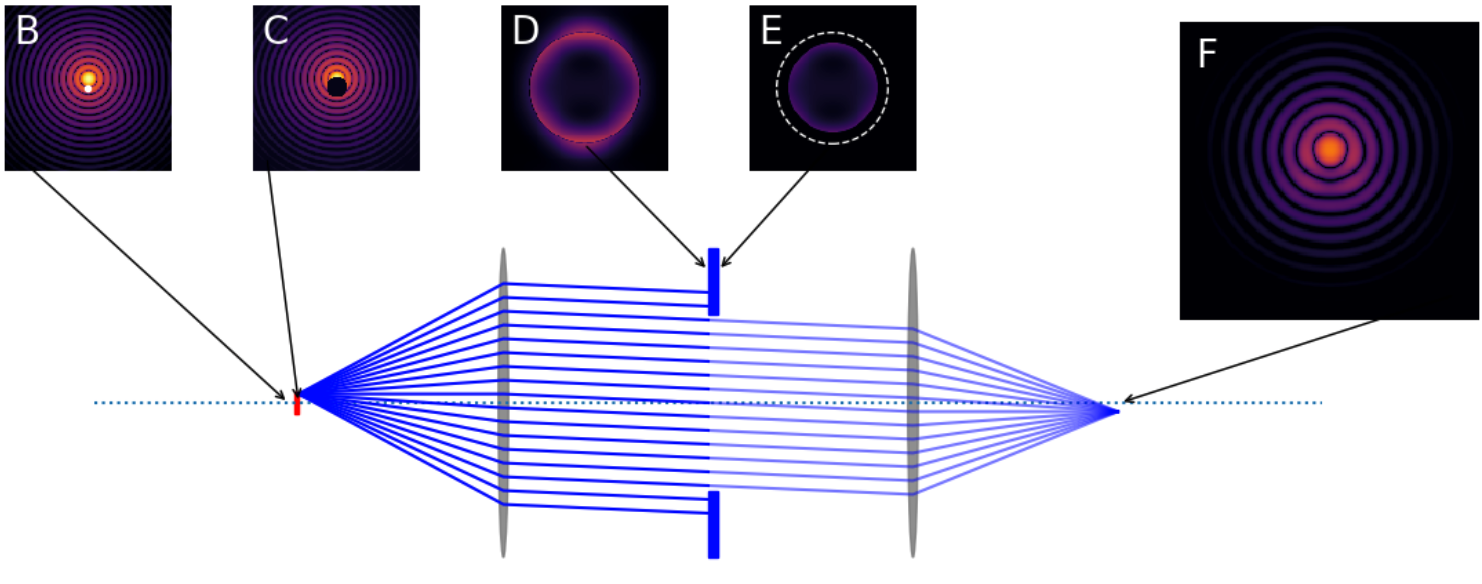
\includegraphics[width=0.95\linewidth]{figures/lyot_coronagraph.png}
  \caption{Lyot coronagraph.
  %
  Geometric rays show the propagation from the \ac{fpm} between B and C, to the Lyot plane at D and E, with the final resultant image at F.}
  \label{fig:lyot}
\end{figure}


\begin{armarginnote}[]
\acc{fpm}
\acc{ppm}
\acc{scfp}
\end{armarginnote}

The first coronagraph to successfully image a debris disk was a Lyot coronagraph built by \citet{Vilas87} and it imaged the edge-on circumstellar disk around Beta Pictoris in 1984 \citep{Smith84}.
%
The optical layout of the Lyot coronagraph can be generalised in Figure~\ref{fig:lyot}, with the letters A-F representing the images present at that location in the coronagraph light path.
%
The telescope pupil (A) is reimaged into a focal plane of the sky (B) where an opaque mask that has high absorptivity and low reflectivity blocks the light from any on-axis source (C).
%
Optics then form an image of the resultant pupil (D) to an intermediate \ac{pp}, where a second opaque mask - the Lyot stop - is located.
%
This Lyot stop blocks the diffracted light of the star - now forming a ring of light along the outer edge of the telescope pupil (E).
%
A second optical system then reimages the resultant focal plane of the instrument onto a detector (F).
%
%When an object is placed behind the focal plane mask, the light from that object is blocked and does not go any further.
%
Any circumstellar objects outside the radius of the \ac{fpm} then pass through unimpeded through the coronagraph and are subsequently reimaged in the detector focal plane at F.
%
The light rays pass through the coronagraph optics to form an image at F with only minor modification: the reimaged pupil at D is superficially very similar to the telescope pupil A.

For an on-axis source, the removal of the Airy core plus attendant diffraction rings significantly modifies the wavefront passing through the coronagraph, resulting in a flux redistribution at D where the flux is concentrated in a ring whose peak brightness lies along the perimeter of the reimaged telescope pupil, extending both beyond the radius of the pupil and into the centre of the pupil.

The purpose of the Lyot stop is to remove as much of this ring of light as possible, whilst maximising the throughput of the pupil image D for off-axis sources.
%
Adjusting the diameter of the \ac{fpm} changes the \ac{fwhm} of the ring of light at D, which requires a smaller Lyot stop to block - but then the throughput of the pupil for off-axis sources then decreases.
%
Decreasing the Lyot stop aperture has a second impact in that the reduced pupil diameter increases the \ac{fwhm} of the images in the final focal plane F, spreading the flux from the off-axis sources over a larger area in the detector and degrading the angular resolution of the telescope and instrument.
%
The optimal diameters of the \ac{fpm} and Lyot stop aperture are then driven by the science requirements - how close to the central star (measured in diffraction widths at the lower spatial resolution) should the coronagraph be able to transmit light from off-axis objects in the field of view.

\section{Parameters to optimize}


\begin{armarginnote}[]
\acc{iwa}
\acc{owa}
\end{armarginnote}

As the previous section explained, clear apertures have solutions that perfectly remove any on-axis light.
%
However, real systems are not ideal and generally don't have a clear aperture.
%
Even more important, stars are not ideal point sources.
%
Solutions that only work for point sources are already out of the question then.
%
The current and future generation of coronagraphs are designed to take on non-ideal environments.
%
This means that the coronagraph is optimized for a specific list of parameters during the design process.

The first set of parameters are the \ac{iwa} and the \ac{owa}.
%
The \ac{iwa} is usually set to the angular separation where the throughput is 50\% of the peak off-axis throughput.
%
The \ac{iwa} and \ac{owa} set the smallest and largest angular separation of the dark hole region that the coronagraph will make.
%
Some coronagraphs, such as the OVC or \ac{fqpm}, don't have an \ac{owa} only an \ac{iwa}.
%
Figure~\ref{fig:coronagraph_focal_plane_definitions} shows a coronagraphic dark hole with the definition of the \ac{iwa} and \ac{owa}.

\begin{figure}[ht]
  \centering
  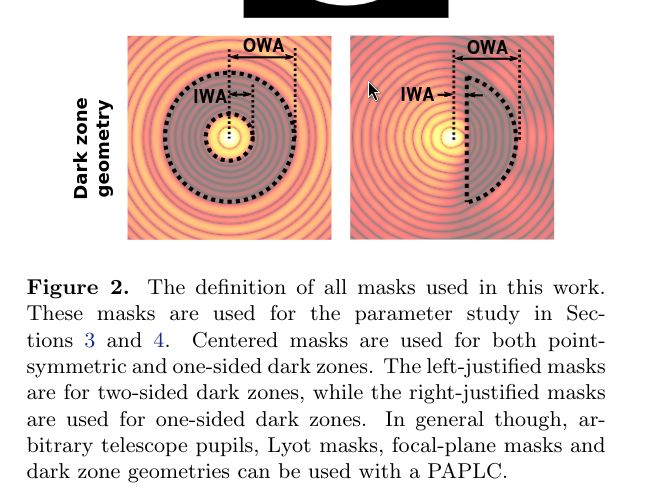
\includegraphics[width=0.5\linewidth]{figures/dark_hole_definition.png}
  \caption{ADD caption \textcolor{red}{TODO: redraw}}
  \label{fig:coronagraph_focal_plane_definitions}
\end{figure}

The contrast and throughput are the next set of parameters that we need to optimize for.
%
The contrast sets the amount of starlight that is left after the coronagraph.
%
It is important to define the term contrast as this can mean many different things.
%
\citet{ruane2018review} provide a thorough overview of the different metrics and their definition.
%
The contrast is defined as
\begin{equation}
C = \frac{\eta_*(\vec{r})}{\eta_p(\vec{r})}.
\end{equation}
Here $\eta_*(\vec{r})$ is the fractional throughput of the star at focal plane position $\vec{r}$ integrated over a photometric aperture.
%
This is then divided by $\eta_p(\vec{r})$ the fractional throughput of the planet in the same photometric aperture.
%
This normalizes the contrast w.r.t. the throughput of the planet, which is important because the planet throughput usually varies as function of angular separation.
%
Both the contrast $C$ and $\eta_p(\vec{r})$ need to be included in the optimization process.
%
The first to make sure that the starlight is nulled and the second to make sure that the planet light is maintained.
%
This optimization has to be done over a certain spectral bandwidth $\Delta \lambda$.

The corongraphs that are designed with only the previous set of optimization targets are not optimal in real environments.
%
In real instrument environments there are wavefront aberrations and small instrumental drifts.
%
These cause light to leak around the coronagraph and cause residual stellar speckles.
%
The coronagraphs must be made robust against low-order wavefront errors and other instrumental drifts.
%
Other more practical things to consider are the precision with which we can align an instrument.
%
For example, how well can the Lyot stop be aligned?
%
The performance of a coronagraph might be extremely sensitive to the Lyot stop alignment, which means that theoretically the coronagraph delivers the contrast but practically it will never reach it.
%
Therefore, alignment tolerancing must be included in the coronagraph design to make sure the target performance is achieved.

In this way, there are many other nuisance parameters that can be included.
%
However, the numerical optimization will take significantly longer if more parameters are included.
%
A good coronagraph designer will therefore make a trade-off between which parameters are required, good to have and not significant.

\section{Beyond Lyot with complex pupil and focal plane masks}


The Lyot coronagraph was designed at the time when it was still difficult to precisely manipulate the phase of light with optics.
%
With the advent of more advanced manufacturing capabilities, very precise phase control became possible.
%
This was a significant boost to the design toolbox for coronagraphs.
%
The major downside of the classic Lyot coronagraph is that only the light that falls on the opaque \ac{fpm} gets blocked.
%
Any light that is off-axis will pass through the system.
%
This holds not only for light that comes from off-axis sources but also for aberrations that causes light to end up outside of the \ac{fpm}.
%
A bigger mask will be able to block a larger fraction of the light and therefore achieve a deeper contrast.
%
However, if the mask is made larger the inner-working angle also becomes bigger and that means fewer planets will be accessible.
%
A smaller \ac{iwa} is crucial both for the extremely large ground-based telescopes and the space-based telescopes. 

We note that the coronagraphic designs in subsequent sections are not optimised but are shown for illustrative purposes.

\subsection{Focal plane phase mask coronagraphs}

Focal plane phase masks offer a solution by phase shifting a part of the \ac{psf} (usually the core of the \ac{psf}) which then causes destructive interference at the Lyot plane.
%
The Lyot stop blocks the areas where the light does not destructively interfere.
%
The 50\% encircled energy radius is on the order of $\sim$\ld{} for almost all aperture shapes.
%
This means that it is possible to achieve perfect destructive interference with a mask that has a size on the order of \ld{}.
%
This is the central idea that was used to design the Roddier and Roddier (RR) phase mask \citep{roddier1997stellar}.
%
The RR mask covers the core of the Airy pattern that contains 50\% of the encircled energy and phase shifts the core by $\pi$ to cause destructive interference.
%
The RR mask works well for monochromatic light, but over broad spectral bandwidths it degrades in contrast.
%
Diffraction causes wavelength scaling of the \ac{psf} that either makes the \ac{fpm} too big or too small compared to the \ac{psf}.
%
Masks made out of multiple concentric rings, such as the dual-zone phase mask \citep{soummer2003achromatic}, were proposed to increase the spectral bandwidth.

\begin{armarginnote}[]
\acc{ovc}
\acc{fqpm}
\acc{agpm}
\end{armarginnote}

Further achromatization for larger spectral bandwidths is possible by designing inherently achromatic phase masks.
%
Inherent achromatic masks are scale invariant, which means that they always look the same regardless of the size of the \ac{psf}.
%
The \ac{fqpm} splits the focal plane into four quadrants and applies a checkerboard $0,\pi$ phase pattern \citep{Riaud00}.
%
The \ac{fqpm} was implemented on the \ac{sphere} instrument \citep{Boccaletti04} and is currently the coronagraph on \ac{jwst} with the smallest \ac{iwa} and has characterized a planet at 1.8 \ld{} \citep{franson2024jwst}. 

If the planet falls on one of the four transition lines between the phases, its transmission is significantly reduced.
%
Increasing the number of phase steps to the continuous limit results in a phase ramp, and this is called the \ac{ovc}.
%
The \ac{ovc} uses a phase mask with a vortex pattern where the phase changes with the azimuthal angle: $\phi=q \cdot \theta$ with $q$ the charge, i.e. the number of times the phase wraps around, of the vortex and $\theta$ the azimuth angle.
%
One implementation of an \ac{ovc} is the \acl{agpm} \citep[\acs{agpm}; ][]{Mawet05b}.
%
This uses subwavelength gratings to impart a charge 2 phase ramp in a \ac{fpm}.
%
The grating manufacture limits the \ac{agpm} to a charge 2 vortex, but higher charges are preferred to make a metter match to the small but finite diameter of stellar disks for nearby stars.
%
A more general challenge is that the \ac{ovs} diffracts all the light out of the \ac{pp} only if the telescope pupil is unobstructed.
%
Secondary support structures and a centrally obscures pupil scatter significant amounts of light back into the \ac{pp}.
%
Suitable Lyots stops can block this stellar leakage, but at a cost of planet throughput.
%
The impact of the central obscuration can be mitigated with the use of a telescope pupil grey apodizer to make a \acl{ravc} \citep[\acs{ravc}; ][]{Mawet13a}.
%
The scale invariant phase masks of these two coronagraphs are shown in Figure \ref{fig:scale_invariant}.

\begin{figure}[ht]
  \centering
  \script{plot_scale_invariant_masks.py}
  \includegraphics[width=0.5\linewidth]{figures/scale_invariant_masks.pdf}
  \caption{The focal plane phase functions of two scale invariant coronagraphs.
  %
  The left figure shows the four quadrant phase mask and the right figure shows the optical vortex phase mask.}
  \label{fig:scale_invariant}
\end{figure}

Both phase masks that are shown in Figure~\ref{fig:scale_invariant} completely null out all on-axis light from a clear aperture.
%
This property is why both the \ac{fqpm} and the \ac{ovc} have been extensively studied over the past several decades.
%
The inner-working angle of both coronagraph approaches 1 \ld{} which makes coronagraphy possible at the diffraction limit!
%

%All ground-based telescopes need to image through Earth's atmosphere. The turbulent nature of the atmosphere causes aberrations that degrade the imaging qualities of the telescope. In such conditions, it is very difficult to optimally reject starlight because what electric field actually needs to be rejected? Is it the electric field that is measured now, or the differently aberrated electric field 20 milliseconds from now? The constantly changing electric field of the incoming light made it difficult to create more advanced coronagraphs. The classic Lyot coronagraph design was not improved upon until the advent of large aperture telescopes with adaptive optics systems that had a high enough performance to deliver diffraction-limited images.
%
%These telescopes made the imaging of low mass substellar companions (brown dwarfs and young self-luminous planets) feasible for the first time.

%
%After the discovery of Gliese 229B (XXX CHECK WAS THIS A LYOT?) with the Palomar 5m PALM 5000 system, a series of coronagraphic designs appeared where researchers explored the different possibilities of placing complex amplitude apodizers at both the focal plane and \ac{pp} locations.
%
%A wide range of coronagraph designs were explored, including XXXXX focal plane, \ac{pp}, telephone list of all different coronagraphs.
%
%MENTION interferometer concepts.


%FINISH 2 SENTENCES SH 



\begin{table}
  \centering
  \begin{tabular}{lll}
    \toprule
    \multicolumn{3}{c}{Comparison of \acs{ppm} and \acs{fpm} coronagraphs} \\[.5\normalbaselineskip]
     & \acl{fpm} & \acl{ppm} \\
    \midrule
    Advantages \\
     & \tabitem Small IWA & \tabitem Pointing invariant \\
     & \tabitem High transmission & \tabitem Single optic \\
     & \tabitem 360 deg FOV & \tabitem Any telescope mirror geometry \\
    Disadvantages \\
     & \tabitem Star diameter leakage & \tabitem Complex manufacture \\
     & \tabitem Pointing sensitive & \tabitem Larger IWA \\
     & \tabitem Complex design with tel pupils & \tabitem Lower planet throughput \\
     & \tabitem Lyot stop required & \tabitem Smaller FOV \\[.5\normalbaselineskip]
    \bottomrule
  \end{tabular}
\end{table}


\subsection{Pupil plane mask coronagraphs}

All stars have a small but finite angular diameter on the sky, typically $\lambda/100$ or less but increasing to $\lambda/10$ for the closest stars.
%R
In the visible, median stars for \ac{hwo} are going to be $\lambda/10$, with some a little larger, becoming even larger as the apertures for \acp{elt} will be larger by a factor of a few: Proxima Centauri has a diameter of 1 mas, which is $\frac{1}{3}$ to $\frac{1}{6}$ \ld{} for the \ac{elt} and the \ac{gmt}.
%
The disk of the star can be treated as a set of incoherent point sources, and so the small but finite angular size of the star means that the sensitivity of contrast of focal plane coronagraphs varies as a function of angle.
%
Given that the star is tens of thousands to millions of times brighter than the target planet, even a small amount of stellar leakage can overwhelm the flux from the planet.


\begin{armarginnote}[]
\acc{sp}
\acc{app}
\acc{gvapp}
\acc{vvc}
\end{armarginnote}


Apodizing the telescope pupil provides an opportunity to redistribute the light in the \ac{scfp} to form `dark zones' around the target star where an exoplanet can be imaged.
%
Strictly this is not so much a coronagraph as a modification to the \ac{psf} of the instrument - all objects in the focal plane have the same \ac{psf}, both stars and exoplanets together.
%
As long as the angular diameter of the star is smaller than the Airy core of the \ac{psf}, \ac{pp} coronagraphs are not impacted by the diameter of the star or by residual tip tilt vibrations that are not removed by the \ac{ao} control loop, making them a robust alternative to the more efficient, smaller \ac{iwa} \ac{fp} coronagraphs. 
%
Suppressing diffraction in the \ac{psf} requires destructive interference using coherent light from the Airy core, but at a cost in Strehl ratio of the \ac{psf}.
%
Since the exoplanet \ac{psf} is identical to the stellar \ac{psf}, the planet throughput decreases too.

The earliest pupil apodizations (referred to as \ac{sp} masks) were with binary amplitude masks \citep{Jacquinot64,Kasdin05} but these had low throughputs, a significant increase in the FWHM of the resultant \ac{psf} (impacting the encircled energy of the planet and the \ac{iwa}) and the limited angular size of the dark zone.
% 
Improvements in the searching of the large dimensional space of possible solutions resulted in the improvement to throughputs of 50\%, working angles of 2.5 to 15 \ld{} and contrasts of $10^{-6}$ \citep{Carlotti11}.
%
Optimizations are also generalised so that they can be designed for arbitrary telescope pupils, so that the secondary obscuration, support structures, and even gaps between segmented mirrors can be accounted for and avoided.
%
Along with their achromatic performance, this makes pupil apodization  suitable for \ac{elt} telescope pupils and enables dynamic coronagraphs using micromachine mirrors \citep{Leboulleux22b,Carlotti23} to account for a dynamically changing pupil (e.g. missing and swapped mirror segments).

Another approach is to apodize in phase only, with the pupil set by the geometry of the telescope pupil \citep{Codona04}; this was realised and subsequently demonstrated on-sky with the Apodizing Phase Plate \citep[APP; ][]{Kenworthy07} which used variations in the thickness of a piece of diamond turned Zinc Selenide to impart a phase shift across the pupil with a central wavelength of 4 microns.
%
An APP built and installed in NAOS/Conica VLT camera \citep{Kenworthy10} led to the first coronagraphic image of Beta~Pictoris~b \citep{Quanz10} and the direct imaging discovery of the exoplanet HD~100546~b \citep{Quanz13}.
%
The original algorithms found solutions with $180^o$ dark `D' shaped regions next to the star, but a more general theory to APP optimisation \citep{Por17}, finds both 180 and 360 degree solutions and additionally finds solutions consisting of regions of integer multiples of $\pi/2$ radians.
%
The first APP optics were chromatic: the OPD was a function of the refractive index of the transmissive material, with the suppression decreasing with increasing bandwidth.

Achromatic phase shifts can be implemented using the principle of geometric phase: the vector-APP \citep[vAPP; ][]{Snik12} replaces the classical phase pattern ($\phi_{\textrm{c}}[u,v] =
n(\lambda) \Delta d[u,v]$) with the ``geometric phase'' \citep[known as the Pancharatnam-Berry phase; ][]{Pancharatnam,Berry}.
%
The vAPP phase pattern is imposed by a half-wave retarder with a patterned fast axis orientation $\theta[u,v]$.
%
The geometric phase is imprinted on incident beams decomposed according to circular polarization state: $\phi_{\textrm{g}}[u,v] = \pm2\cdot\theta[u,v]$, with the sign depending on the circular polarization handedness.
% %%%
As this fast axis orientation pattern does not vary as a function of wavelength (with the possible exception of an inconsequential offset/piston term), the geometric phase is strictly achromatic.
%
%A simple Fraunhofer propagation from the pupil $[u,v]$ to the focal plane $[x,y]$ shows that after splitting circular polarization states the two ensuing coronagraphic \ac{psf}s are point-symmetric ($\ac{psf}_{\textrm{L}}[x,y] = PSF_{\textrm{R}}[-x,-y]$), and therefore, in the case of D-shaped dark holes, delivers complementary PSFs that furnish instantaneous $360^\circ$ search space around each star.
%
Vector-APP devices are produced by applying two liquid-crystal techniques: any desired phase pattern is applied onto a substrate glass through a \textit{direct-write procedure} \citep{directwrite} that applies the orientation pattern $\theta[u,v]$ by locally polymerizing the alignment layer material in the direction set by the controllable polarization of a scanning UV laser.
%
Consecutive layers of birefringent liquid-crystal are deposited on top of this alignment layer, which subsequently self-align \citep[``\textit{Multi-Twist Retarders}''; MTR ][]{MTR} with predetermined parameters (birefringence dispersion, thickness, nematic twist) to yield a linear retardance that is close to half-wave over the specified wavelength range.
%
Additional layers broaden the wavelength range to over an octave in wavelength, at a cost of an absorption feature due to the carbon-carbon bonds within the liquid crystal and glue layers.
%
The vector-APP devices required additional optics (typically a half-wave plate and Wollaston prism) to isolate the two circular polarizations and produce two separate \acp{psf} with dark holes on opposing sides of the central star \citep{Snik12}.
%
By adding a phase diffraction grating onto the APP phase pattern to make a grating vector APP \citep[gvAPP; ][]{Snik12,Otten14}, the other optics are no longer required.
%
The two coronagraphic \acp{psf} are separated diffracted into the $m=\pm 1$ order, with a $m=0$ ``leakage term'' non-coronagraphic \ac{psf} with flux of a few percent of the original star left in the undeviated beam, acting both as an astrometric and photometric reference \citep{Otten17,Sutlieff24}.
%
The grating effect means that the \ac{psf} centroids vary as a function of wavelength, and so the gvAPPs are ideal for imaging onto integral field units and image slicers \citep{Sutlieff21,Sutlieff23}.
%
This liquid-crystal technology has enabled coronagraphic designs that were previously impossible to manufacture, including the coronagraphic modal \ac{wfs} \citep{Wilby17}, Sparse Aperture Masking with multiple holograms \citep{Doelman21}, complex amplitude Vector Vortex Coronagraphs \citep[VVC; ][]{Snik14}, and triple grating coronagraphs \citep{Doelman20} that redisperse the \acp{psf} back into white light coronagraphic \acp{psf} for VVCs \citep{Doelman23,Laginga24}. 
%
A comprehensive review of the coronagraphs enabled by the liquid crystal technology is given in \citet{Doelman2021a}.

\section{Apodized Lyot Coronagraphs}\label{sec:nulled_lyot}

The fundamental goal of any coronagraph is to block the light from the star, while passing through the light of the planet. Any type of \ac{fpm} coronagraph, like the Classic Lyot coronagraph, will find that it is very difficult to completely null out the star. This is due to a mismatch between the modes of the incoming electric field from the aperture and the \ac{fpm} filtered electric field.
%
The propagation through a Classic Lyot style coronagraph can be described by two propagations. The first is a propagation through the area that is covered by the mask itself, $m_1$, and the second is the negative of the mask $m_2$. Together, these two masks cover the full focal plane. The propagation of the electric fields then follow as,
\begin{equation}
    E_{\mathrm{out}} = t\invfourier{m_1 \fourier{E_{in}}} + \invfourier{m_2 \fourier{E_{in}}}.
\end{equation}
Now let's simplify this by substituting $\hat{m}=\fourier{m_1}$, $m_2 = 1 - m_1$ and using the Fourier convolution theorem. This results in a simplified equation,
\begin{equation}
    E_{\mathrm{out}} = E_{in} + (t-1)\hat{m}*E_{in}.
\end{equation}
The output is the sum of two electric fields, the original input electric field and a filtered electric field. The filtered light is allowed to diffract light outside the geometric pupil because this is blocked by the Lyot stop. Therefore, the condition for perfect nulling is found by setting the output over the geometric pupil to zero. 
\begin{equation}
    E_{in} + (t-1)\hat{m}*E_{in} = 0.
\end{equation}
This condition can only be fulfilled if the incoming electric field is an eigenfunction of the filtering operator.
\begin{equation}
    \hat{m}*E_{in} = \gamma E_{in}.
\end{equation}
Then
\begin{equation}
    E_{in} + (t-1)\gamma E_{in} = 0,
\end{equation}
and a perfect null is achieved when $(t-1)\gamma = -1$. The normal pupil illumination is uniform and is not an eigen function of the filtering operator. Therefore, it is not possible to perfectly null the starlight with any type of Lyot-style \ac{fpm}. The apodization profile for several different telescope apertures and \ac{fpm} diameters are shown in Figure \ref{fig:fpm_eigenfunctions}. These eigenfunctions are Prolate Spheroids and they generate theoretically perfect nulls if combined with the Roddier \& Roddier coronagraphs \citep{soummer2003stellar}.

\begin{figure}[ht]
  \centering
  \script{plot_scale_invariant_masks.py}
  \includegraphics[width=\linewidth]{figures/fpm_eigenfunction.pdf}
  \caption{The pupil amplitude distribution that are eigen functions of certain \ac{fpm} sizes. The top row is the unapodized pupil function, which is the pupil eigenfunction for an infinite \ac{fpm} size. The middle and bottom rows show the eigenfunctions for a 1 and 2 \ld{} \ac{fpm} diameter, respectively. Each column represents a different telescope with from left to right; a clear aperture, the VLT, the \ac{gmt} and finally the ELT.}
  \label{fig:fpm_eigenfunctions}
\end{figure}

The incoming pupil amplitude must therefore be apodized. This insight led to the development of various coronagraphs with different combinations of phase/amplitude pupil apodization and opaque/phase shifting \acp{fpm}.

\subsection{The Apodized Pupil Lyot Coronagraph (APLC)}
The first modification of the Lyot coronagraph that people experimented with was the \ac{aplc}. The \ac{aplc} uses achromatic grey-scale pupil apodizers to better match the entrance amplitude distribution to the \ac{fpm}. These coronagraphs are quite robust and in use in many different high-contrast imaging instruments such as \ac{sphere} \citep{beuzit2019sphere}. Currently, there is still active research in the optimization strategies for the \ac{aplc} such as for future segmented space telescopes \citep{zimmerman2016lyot} and for upgrades of ground-based instruments \citep{nickson2022aplc}. The major downside of the \ac{aplc} is the lower transmission due to absorption in the apodizer.


\subsection{The Phase Apodized Pupil Lyot Coronagraph (PAPLC)}
\label{sec:paplc}
%Emiel came up with concept, 2019, has unpub paper and SPIE talk...
Phase apodization instead of amplitude apodization is twice as effective in improving the performance of the Lyot Coronagraph \citep{Por20}. This comes from the range of allowed apodization values. Instead of being limited between $[0, 1]$, it is possible to use phase offsets to increase the range to $[-1, 1]$. And, it also allows for complex value apodization. The solutions for circular dark holes are found to be discretized; the phase is either 0 or $\pi$ \citep{Por20}. This reminiscent of the solutions found for optimal APPs \citep{Por17} and binary shaped pupils \citep{Carlotti11}. Full circular dark holes are not very efficient since they require strong phase patterns to create the dark holes which causes significant Strehl loss \citep{Por17}. One-sided dark holes are much more efficient in terms of Strehl. 

Talk about the stark paper \citep{Stark24} full end to end yield simulations.

Mention that this is the baseline for GMAGAOX (find 2024 SPIE Males paper).
%Haffert 2023 paper

They have been implemented in the lab - SCOOB 2021 AZ space test bed \citep{Ashcraft22} using a knife edge SPIE proceeding. \ac{aplc}. \citep{vanGorkom22}.

\subsection{The Hybrid Lyot Coronagraph (HLC)}

Mention the Roman design.

The first optimised coronagraph in space!


\subsection{The Phase Induced Amplitude Apodization Complex Mask Coronagraph}

Phase Induced Amplitude Apodization (PIAA) remaps the telescope pupil such that a star on the optical axis forms a \ac{psf} with no diffraction rings - typically a 2-D Gaussian profile \citep{Guyon03,Guyon05,Guyon14}.
%
The pupil remapping optics can be either transmissive or reflective, with reflecting optics more amenable to achromatization but more challenging to manufacture.
%
The optics induce aberrations for off-axis sources that are strong functions of increasing distance from the optical axis, significantly decreasing the Strehl ratio of these sources and lowering their effective sensitivity.
%
A reimaging system that reverses the optical aberrations of the first set of PIAA optics then reforms a final focal plane image with all off axis sources forming diffraction limited images.
%
An on-axis \ac{fpm} then blocks the starlight whilst allowing off-axis sources to propagate through to the final focal plane.
%
The original design (PIAAC) uses a hard edged apodizer, but by allowing the design to include other coronagraphs (an amplitude apodized Lyot coronagraph; AALC) or a complex mask coronagraph (CMC), they can approach the ideal coronagraph in their suppression - see Figure~\ref{fig:piaatypes}.

\begin{figure}[ht]
  \centering
  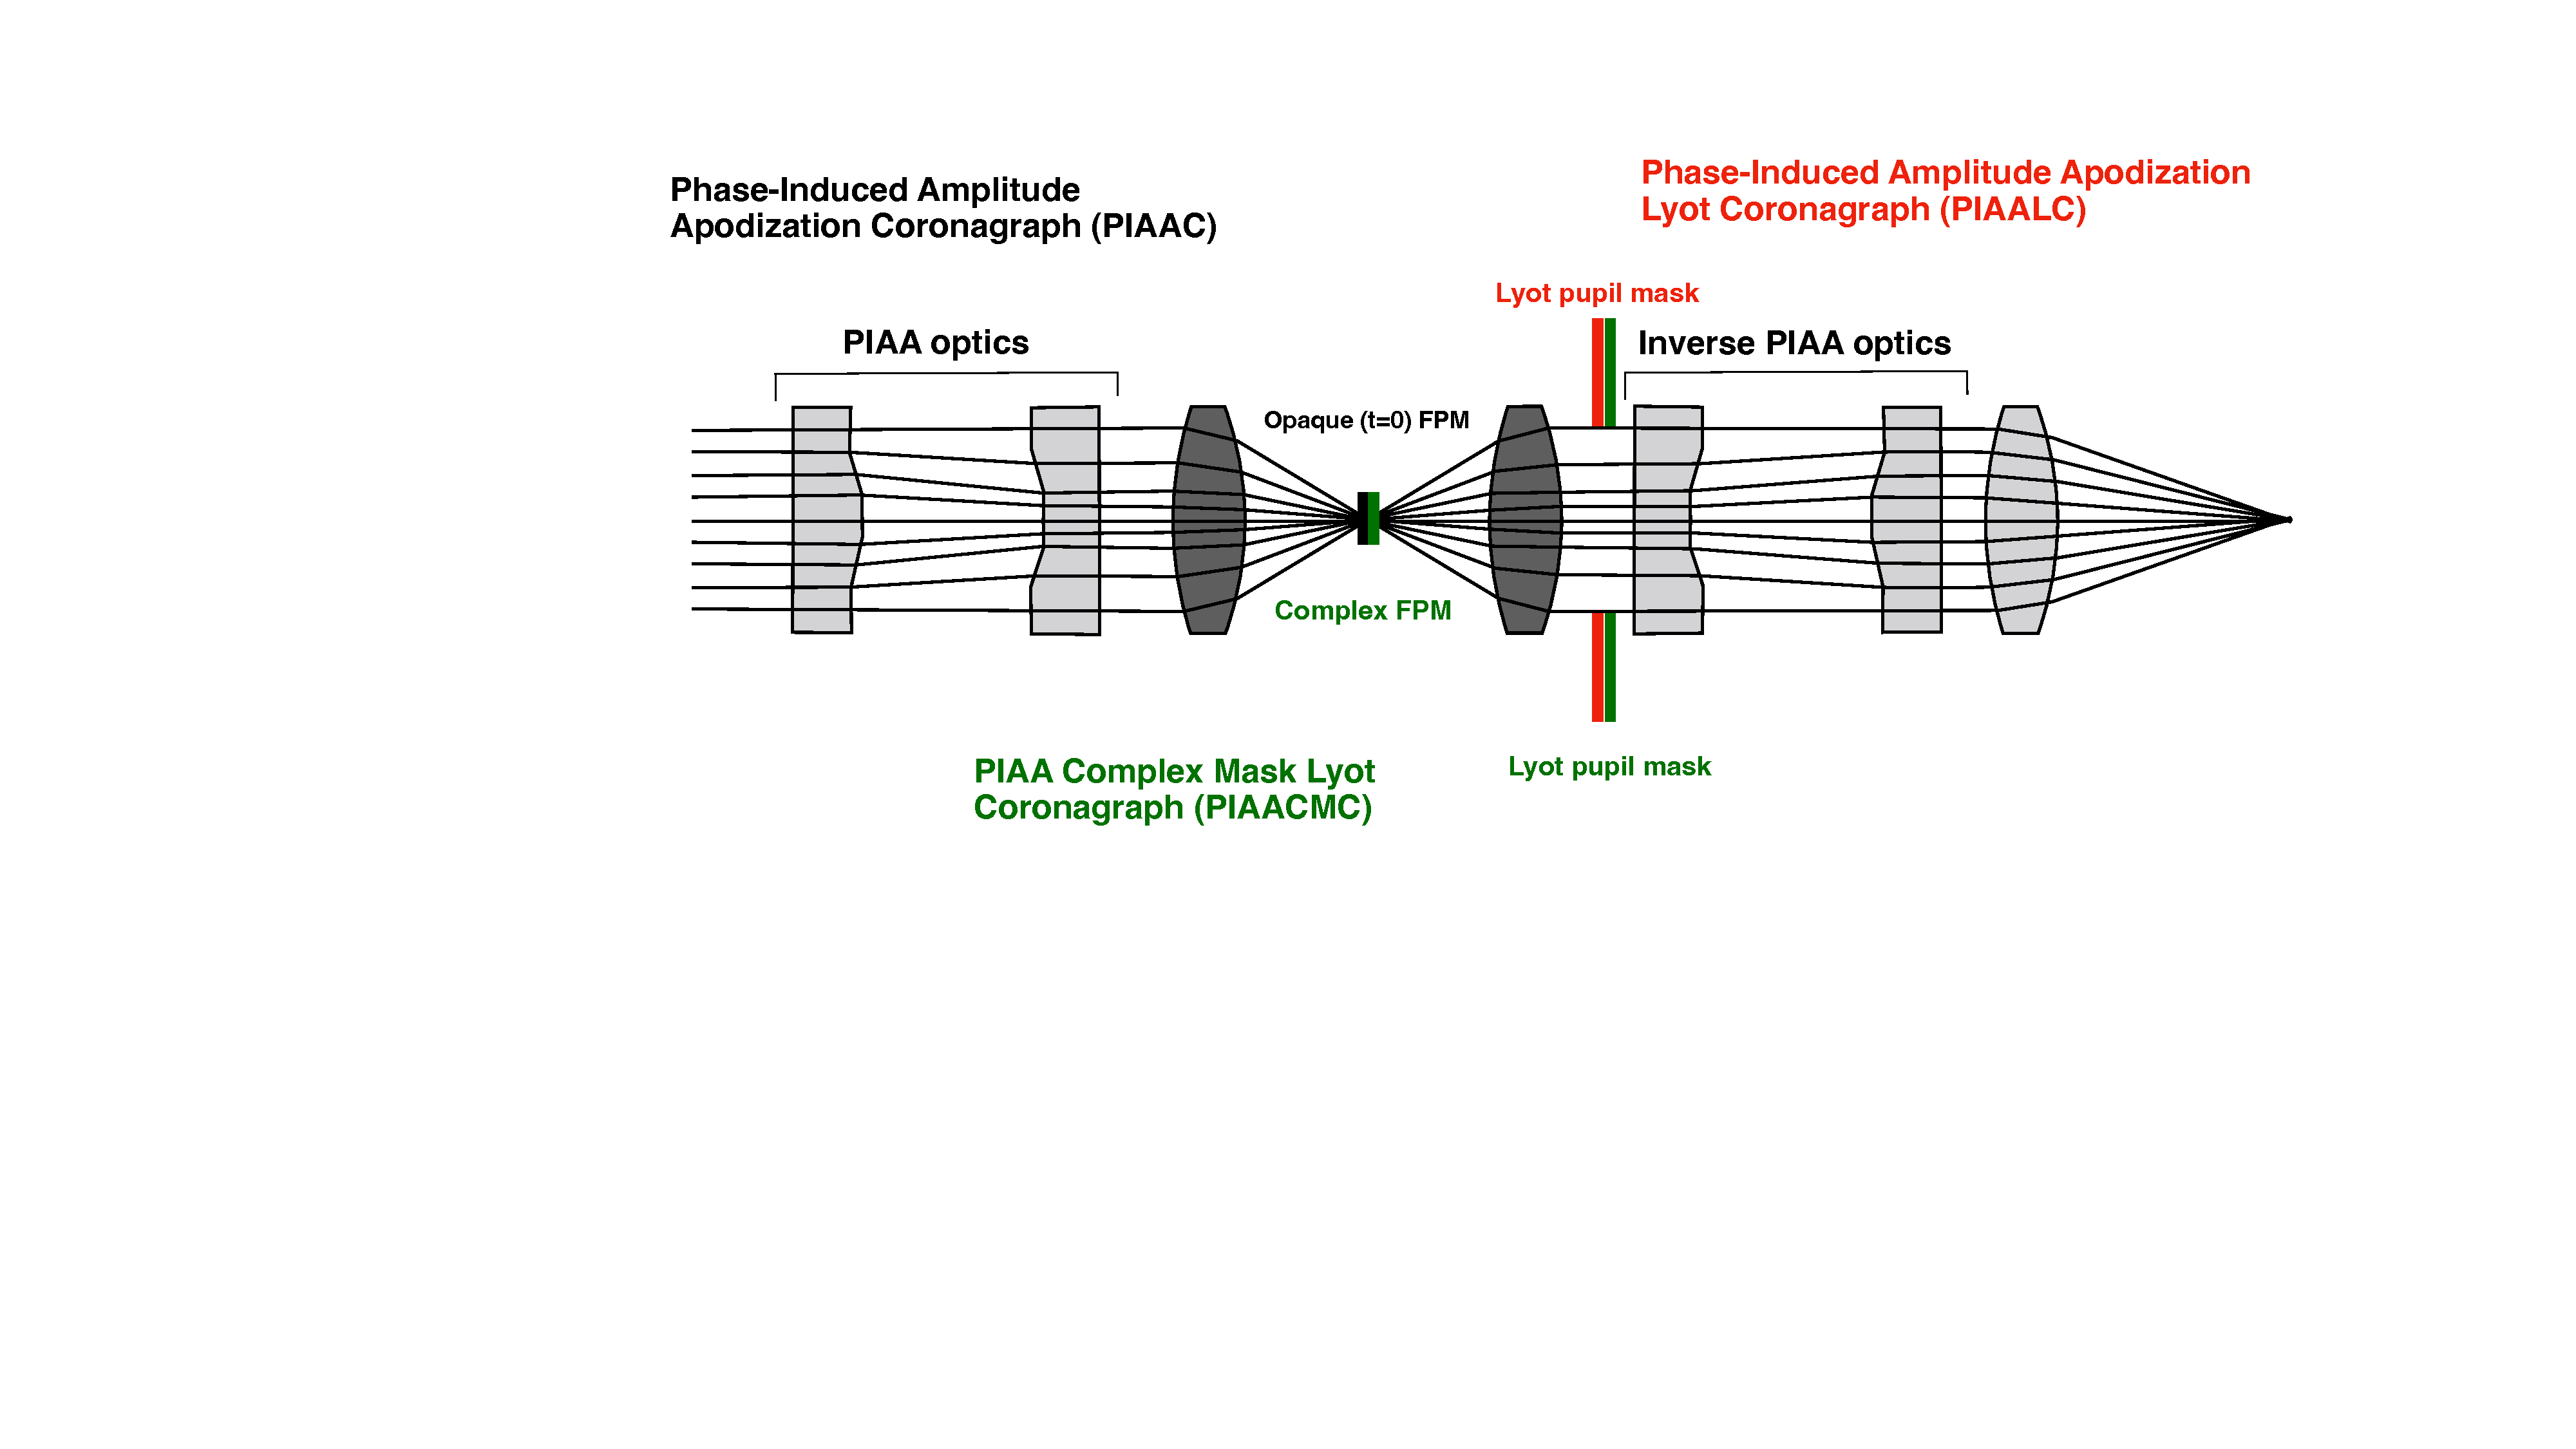
\includegraphics[width=0.9\linewidth]{figures/piaas.pdf}
  \caption{Different types of PIAA coronagraph. Adapted from Guyon 2011 SPIE paper.}
  \label{fig:piaatypes}
\end{figure}

%The PIAA system approaches the ideal coronagraph limit, making it a compelling choice for small IWA coronagraphs.
%
Original PIAA designs are for unobscured circular apertures: telescope pupils with secondary obscurations require additional formatting of the pupil to make a continuous diffraction-free \ac{psf} in the coronagraphic focal plane.
%
The introduction of complex masks that can be manufactured to the required tolerances enable PIAAs for complex and segmented telescope pupils, suitable for space-based telescope designs such as the HabEx/LUVOIR concepts.
%
Results from the laboratory demonstration of a Phase-Induced Amplitude Apodization Complex Mask Coronagraph (PIAACMC) coronagraph with a segmented aperture, \citep{Marx21}, show contrasts of XXXX at YYYY with ZZZZ bandwidth.
%
Most recently, the laboratory demonstration of high contrast with the PIAACMC coronagraph on an obstructed and segmented aperture \citep{Belikov22} shows YYYY contrast achieved.

Ultimately the rejected light can form the basis for a \ac{wfs} to keep the PIAA pointed and aligned with the science target, and an integrated \ac{wfs} and coronagraph with PIAACMC has been demonstrated \citep{Haffert23a}.


\section{Spatial mode demultiplexing}

The principle of \ac{smd} is to use waveguides as modal filters on the complex electric field to separate them into different optical pathways.
%
An early example is the filtering of the input of a nulling interferometer.
%
Two subapertures from a wavefront are brought to a focus with a $\pi$ radian phase shift between them, forming a set of Young's fringes on the sky with an on-axis stellar source nulled out quadratically.
%
The electric field of the fringes are antisymmetric, with the complex electric field changing sign across the central null.
%
By using a single mode fiber at the focus  which only permits transmission of the lowest electromagnetic mode of the circular aperture of the fibre (HE$_{11}$), the sign change of the (point anti-symmetric) electric field results in a deep null, and wavefront aberrations are minimised \citet{Serabyn06,Haguenauer06}.
%
Any planet that is sitting in an adjacent transmissive region of the fringe pattern (and is on the face of the fibre) has a point symmetric electric field, and will couple into the fiber, albeit with a reduced transmission.

This principle is used to minimise the contribution of speckles in the focal plane at the location of the planet, where the Airy core of the planet is injected into a single mode fibre \citep{Mawet17}.
%
High coupling efficiency is possible (with a theoretical maximum of 81\% for an Airy core into the Gaussian HE$_{11}$ mode) and reflected light around the fibre used to sense and minimise speckles whilst the incoherent light of the planet remains constant and injected into the fibre.

The \ac{ovc} has a planet throughput of 0.7 at 1 \ld{} of the on-axis null \citep{Mawet05b}, and placing an optimally matched single mode fibre at the location of the null provides suppression of the star much greater than the transmission loss of the coronagraph for a planet at 0.5 to 1\ld{} from the star, resulting in a peak transmission of 0.2 at 0.9 \ld{}.
%
This principle is called \acl{vfn} \citep[\acs{vfn}; ][]{Ruane18} and different telescope pupils with both \ac{pp} and \ac{fp} \ac{ovc} are explored in \citet{Ruane19}, with on-sky results demonstrated in \citet{Echeverri24}.

The \ac{vfn} provides almost no information on the azimuthal position of the planet, and because it is off-axis it does not couple with the highest efficiency.
%
One solution is to use a \acl{mspl} \citep[\acs{mspl}; ][]{LeonSaval13}.
%
This replaces a single-mode fiber with a cluster of fibres in a close-packed configuration that optimally match the focal plane with a \ac{ovc}.
%
The properties of the coupling increase the planet throughput and partial localisation of the planet \citep{Xin22}.
%
The \ac{vfn} and \ac{mspl} feed high dispersion spectrographs to perform \ac{hci} \citep[][ and this Review]{Snellen15}, where the speckle field changes slowly with wavelength and can be approximated as a constant background over limited wavelength ranges.

\ac{smd} can also suppress the diffraction halo of a star by using a single mode fibre that has a diffraction null crossing the face of the fibre.
%
The sign change in the electric field across the null means that a fibre centered on the null has a significantly reduced electric field propagated through the fibre, but the Airy core of the planet will couple with high efficiency.
%
This technique works in the narrow band, but since the diffraction halo scales radially with \ld{}, the null line no longer passes through the centre of a fibre that is offset from the optical axis defined by the star.
%
The effect can be made to work across a significantly wider bandwidth by having two successive nulls cross the fibre area: as the two nulls move out radially with wavelength, the two sign changes across each null compensate each other to first order.
%
An \ac{app} with modest apodization can be made to squeeze two null crossings closer to each other, and using a hexagonal lenslet array matched to the circular single mode fibres enables a high efficiency transmission of planet flux through to the spectrograph, but with a large bandwidth called \acl{scar} \citep[\acs{scar}; ][]{Por20a,Haffert20}.
%
This principle has been demonstrated in laboratory experiments with 360 degree and 180 degree  dark regions from 0.8–2.4 \ld{} around the star \citep{Haffert20}.
%
In these experiments, the 360 SCAR was designed for an unobscured telescope pupil and created a measured stellar null of $2-3 \times 10^{-4}$, and a 180 SCAR was designed for a telescope aperture with central obscuration and spiders and reached a null of $1\times 10^{-4}$. 

\todo{figure from SCAR paper showing arrangement of the APP and fibres}

\section{Wavefront Sensing and Correction}

The coronagraph designs assume that the incoming wavefronts from all the astrophysical sources in the field of view are flat, and that the optics in the coronagraph are ideal, propagating and modifying these wavefronts without distortion to the final \ac{scfp}.
%
In reality, however, there are several factors that cause deviations of the wavefronts from this ideal: (i) optical manufacturing limitations, (ii) environmental conditions (both static and dynamic) within the instrument and the telescope, and in the case of ground based telescopes, (iii) the wavefront residuals from the Earth's turbulent atmosphere partially corrected with a high order adaptive optics system.

\subsection{Adaptive Optics}

Adaptive optics sense the turbulence introduced by the Earth's atmosphere $\phi_{TURB}$ using Wavefront Sensors which measure a wavefront $\phi_{WFS}$, reconstruct an estimate of this turbulence $\phi_{CALC}$, and use an electronically actuated deformable optical element - typically a \ac{dm}\footnote{There are several other optomechanical devices that exploit other optically active principles to modify a wavefront.} - within the instrument to modify the incoming turbulent wavefront and flatten it.
%
With the \ac{dm} upstream of the WFS, and an \ac{ao} computer providing the calculation of wavefront measured by the \ac{wfs} and applying this correction $\phi_{CALC}$ to the \ac{dm}, this forms a {\bf closed loop}, where the response of the \acp{dm} correction is seen by the \ac{wfs} in the instrument, see Figure~\ref{fig:aosystem}.
%
The fundamental limits in \ac{wfs} are discussed in .

%
\begin{armarginnote}[]
\acc{dm}
\acc{fpm}
\acc{ppm}
\acc{wfs}
\acc{ao}
\end{armarginnote}

Incoming light is split using a dichroic or grey beamsplitter, sending some of the light to the science camera and the rest to the \ac{wfs} camera.
%
Many \ac{ao} systems take advantage of the fact that the optical path difference (OPD) introduced by the Earth's atmosphere above ground based telescopes is achromatic, despite OPD amplitudes of several tens of microns across large telescope apertures.
%
A consequence is that a wavefront measurement at a shorter wavelength (typically at optical or NIR wavelengths) will provide correction for all longer (science) wavelengths.
%
For 8m class telescopes looking at bright stars, when the wavefront sensing is carried out at the same wavelength as the science camera $(\lambda_{WFS}=\lambda_{SCI})$, the theoretical contrast is $10^{-6}-10^{-7}$ but when $\lambda_{WFS}$ is in the optical and $\lambda_{SCI}$ is in the infrared, the limit is set by the scintillation chromaticity induced by Fresnel propagation through the atmosphere to $10^{-4}-10^{-5}$ within one arcsecond \citep[see ][ for a discussion of this and the other limits to \ac{ao} for HCI]{Guyon05-1}.

\begin{figure}[!ht]
\centering
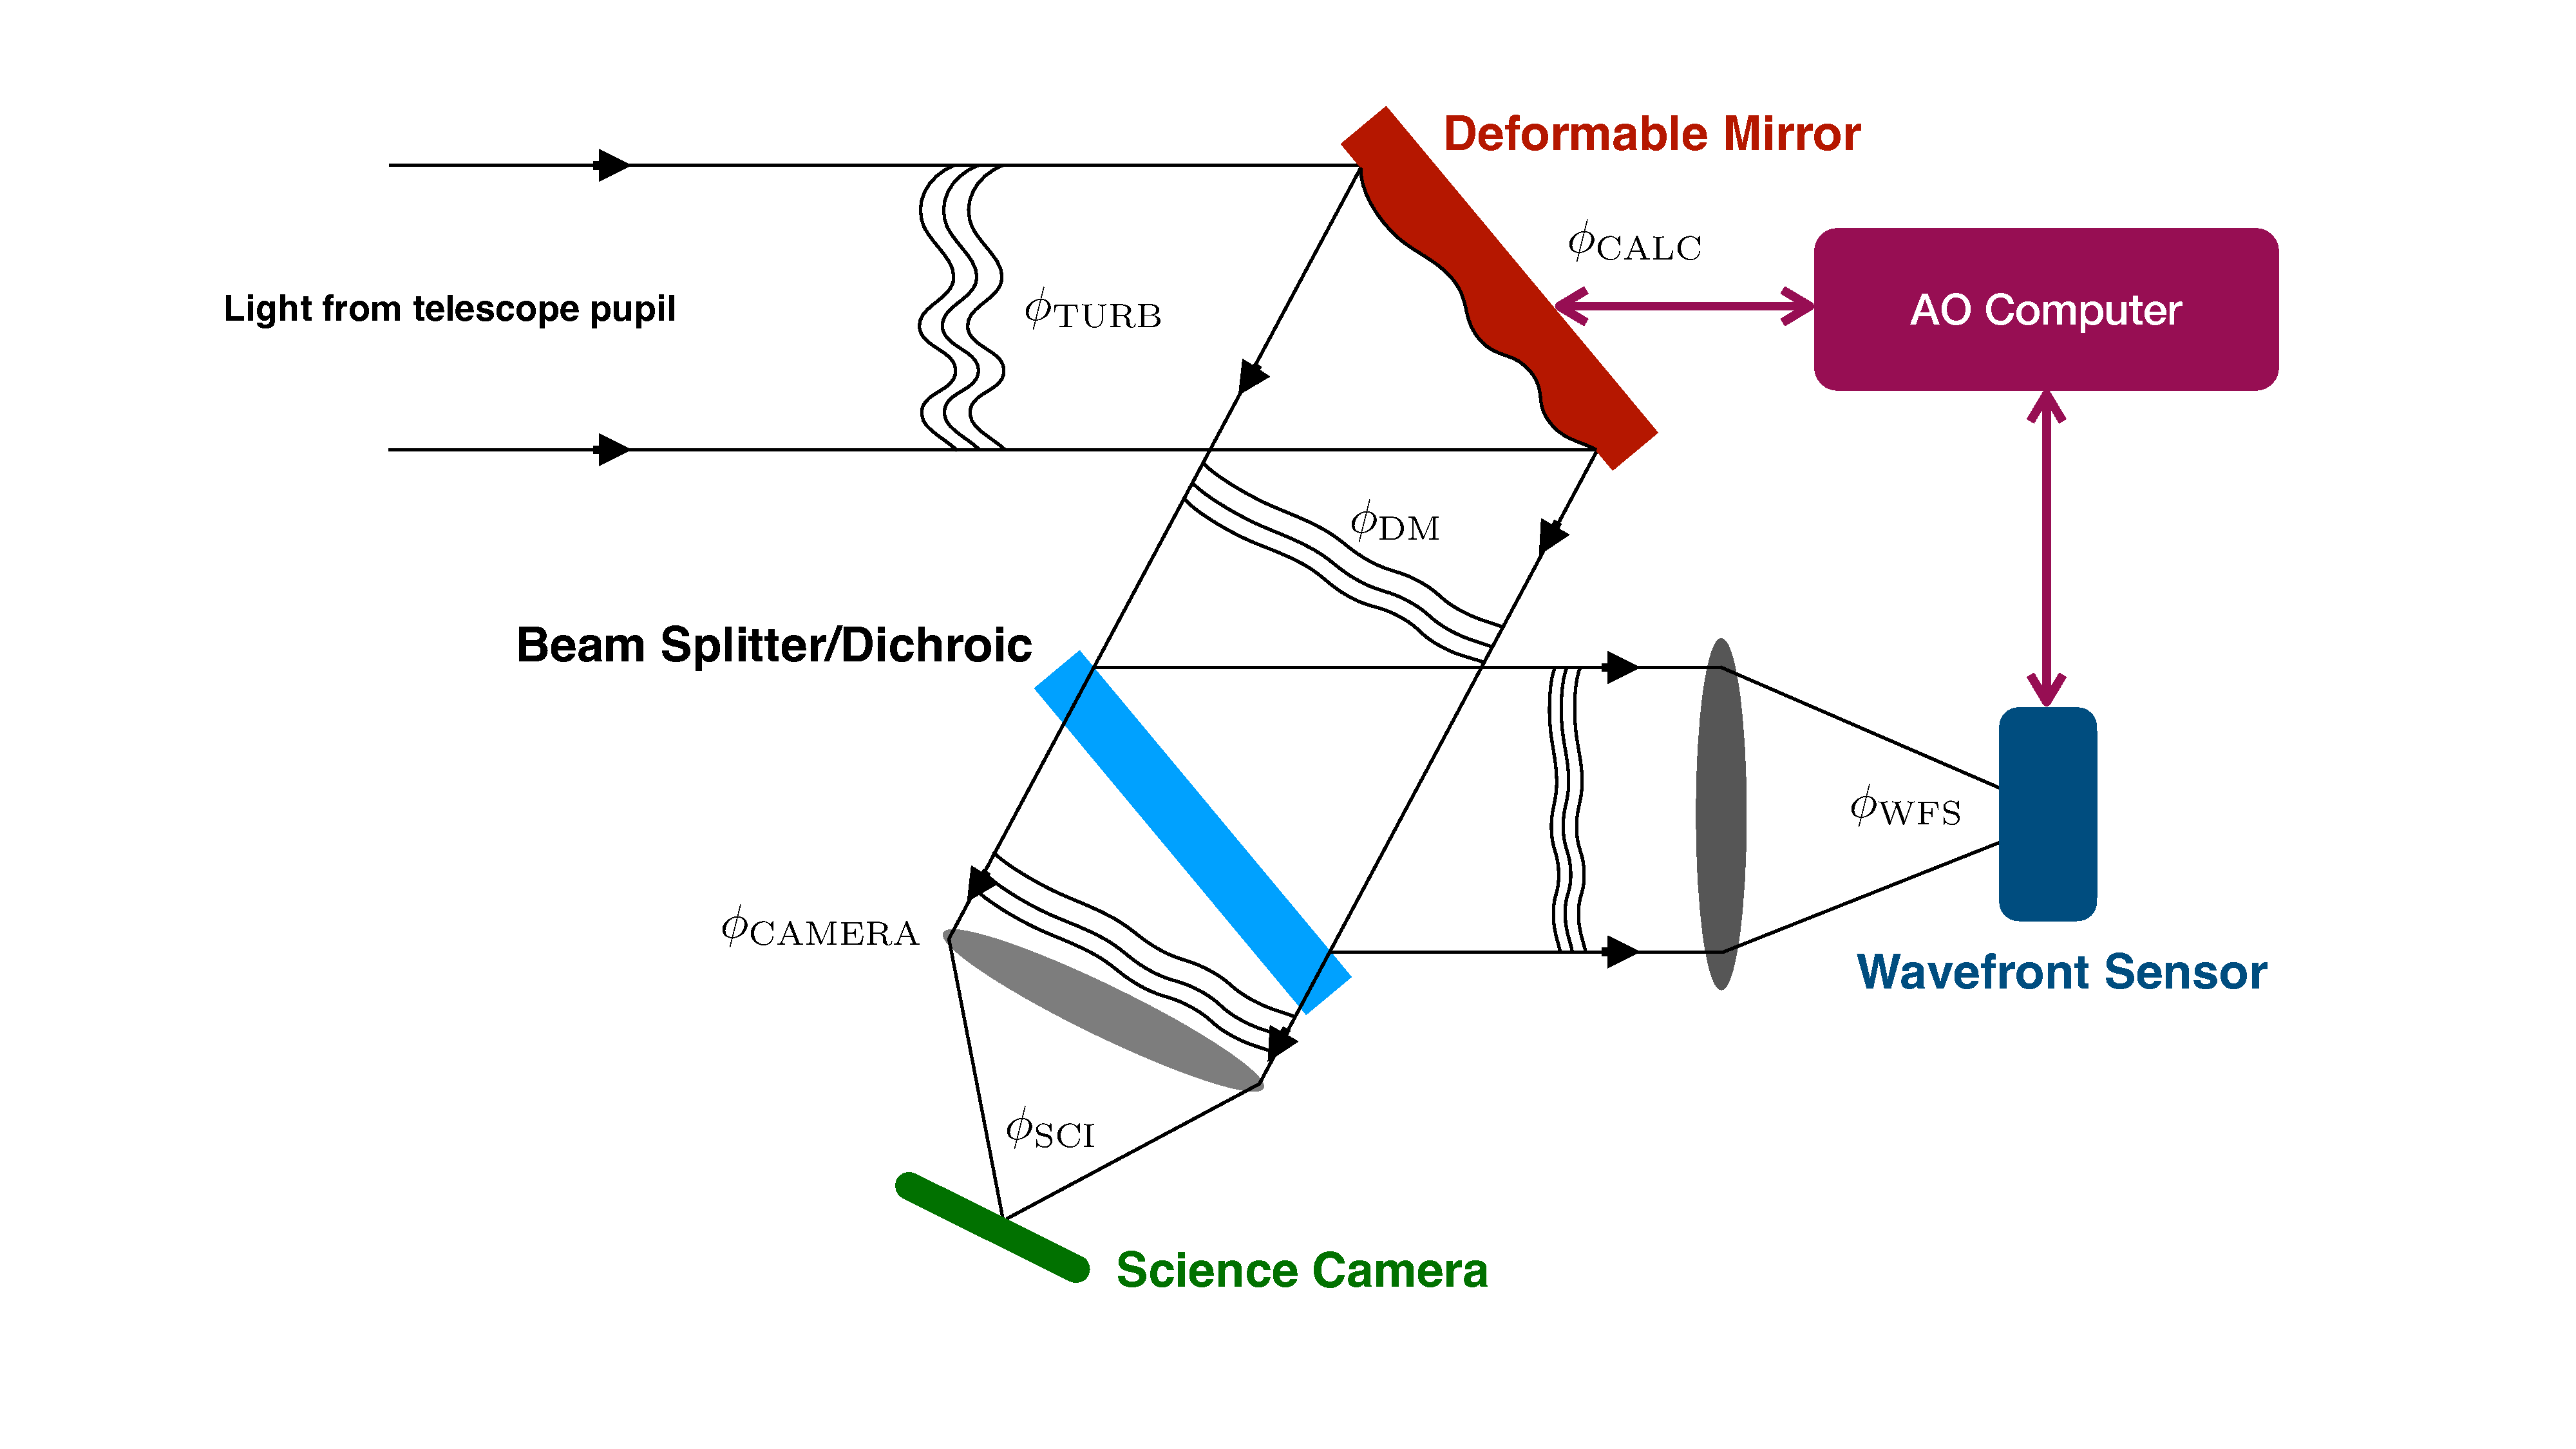
\includegraphics[width=0.9\linewidth]{figures/ao_system.pdf}
 \caption{\ac{ao} system schematic. The incoming turbulent wavefronts are reflected off a \ac{dm}, then a beamsplitter sends some of the light to a \ac{wfs}, and the remaining light passes to the science camera. An \ac{ao} computer takes the measurements from the \ac{wfs}, reconstructs the measured wavefront, and sends a correcting signal to the \ac{dm} to flatten the incoming wavefront.}
  \label{fig:aosystem}
\end{figure}

The Earth's atmosphere is highly dynamic and changes on a timescale of milliseconds, but the wavefront reconstruction and correction on the \ac{dm} is not instantaneous, leading to a small but significant time lag between measurement and the application of the correction.
%
Adaptive optics is a complex and mature field in its own right, covering atmospheric turbulence, optomechanics, engineering control theory, wavefront sensing and information theory (each of these topics would be a review in their own right), but for now we refer the reader to \citet{Guyon18} for reviews on these topics. 
%
For our purpose, we assume that ground based instruments have a high order adaptive optics system providing high order wavefront correction, resulting in a time evolving screen of residual phase errors that change on a timescale of milliseconds and have $\lambda/20$ r.m.s.

We simulate a typical 8m telescope high order \ac{ao} system feeding a high contrast instrument that contains an ideal coronagraph: the \ac{dm}has 40 actuators across its diameter, resulting in a control halo 20 diffraction widths in diameter. 
%
The closed loop speed of the \ac{ao} system is 1kHz, with \ac{wfs} observing at 0.5 microns and the science camera wavelength of 1.65 microns.
%
A single layer of turbulent atmosphere with $r_0$ of $2m$ at 2.2 microns and speed 10 m/s is simulated to show the presence of the wind-driven halo.
%
In Figure~\ref{fig:ao}, a plume of speckles is seen around the central image, a result of the unsensed atmosphere entering the telescope pupil before it is corrected by the \ac{ao} system. 
%
Instantaneous speckles average out over time to an azimuthally symmetric halo, with an extended wind-driven plume that can be time varying in orientation and even asymmetric in the presence of strong turbulence \citep{Cantalloube18}.

% https://docs.hcipy.org/dev/tutorials/ShackHartmannWFS/ShackHartmannWFS.html

\begin{figure}[ht]
  \centering
  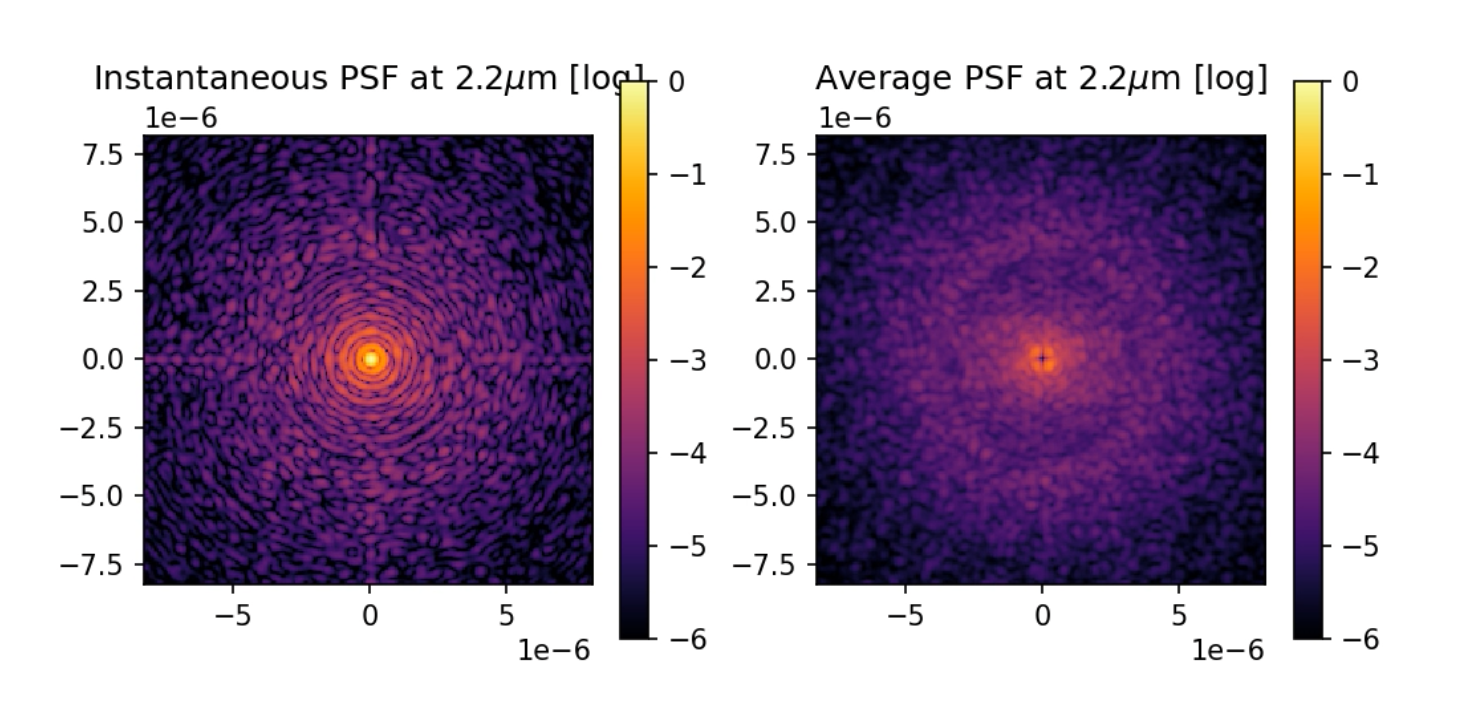
\includegraphics[width=0.9\linewidth]{figures/ao.png}
  \caption{Closed loop of an \ac{ao} system showing features from the loop \textcolor{red}{TODO: label up halos and run for longer}}
  \label{fig:ao}
\end{figure}

\subsection{Non-Common Path Aberrations}

Aberrations can be sensed and corrected to the point of the last \ac{wfs} in the optical path in the high contrast instrument.
%
Ideally the sensed wavefront $\phi_{WFS}$ is identical to the wavefront delivered to the science camera $\phi_{SCI}$, but since the wavefront is split at the beamsplitter, there is a difference in the \ac{wfs} wavefront and the Science camera wavefront.
%
The differential aberrations between this \ac{wfs} and the final \ac{scfp} are referred to \acp{ncpa}.
%
\acp{ncpa} are time varying over a wide range of timescales, with lab based measurements showing decorrelation timescales from seconds to minutes and hours \citep{Martinez12,Males21}.
%
First generation HC instruments provided little to no active \ac{ncpa} measurement and in-situ mitigation strategies, but the presence of \acp{ncpa} were a significant impact on the sensitivity of these instruments at smaller \ac{iwa}, reducing the predicted contrast from their designs.
%
Subsequent instruments have taken multiple approaches to \ac{ncpa} at every stage of the instrument's life cycle:

\begin{itemize}
    \item BEFORE the instrument is built: Minimising the number of optics that can contribute to the \ac{ncpa} \citep[by making the optics optomechanically and thermally stable; ][]{Absil24}.
%    \item Predictive control and speckle lifetime \citep{Males18}. 
    \item DURING the science camera exposures: Developing methods for estimating the wavefront at the final \ac{scfp} and providing in-instrument feedback.
    
    \item AFTER the data is taken: Developing algorithms that provide estimates of the science camera \acp{psf}s at all times during the science camera exposure (REF review)

\end{itemize}

XXXX

Macintosh 2005, and Hinkley 2000 with timescales

\todo{need figure showing decorrelation with time on some system....}

%Jared's AO4 \ac{elt}paper was a good talk, but this is the argument to limit to 30 parsec.

%Haffert 2023 talk mentioned this ore we can talk about it below:

%Diffraction limit of telescope is almost fundamental limit. The HZ stays fixed in linear space, but the angular size shrinks with distance of star from Sun.

%Apparent magnitude of the stars goes down, \ac{ao} performance goes down, halo fills in.

%Jared and Guyon 2018/19 on predictive control and speckle lifetime - \citep{Males18}

%Jared 2020 speckle lifetime \citep{Males21}

%Self coherent camera (Pierre? Baudoz 2006 original \citep{Baudoz06}) refael Galicher paper from 2010 instead/as well Self-coherent camera as a focal plane wavefront sensor: simul .


\section{Challenges for Segmented Telescopes}

The Extremely Large Telescope projects are the European ELT, the Thirty Meter Telescope and the Giant Magellan Telescope.
%
All three telescopes have altitude/azimuth mounts, with segmented primary mirrors that have support structures holding a secondary mirror in front of the primary, blocking the central part of the telescope pupil.
%
The telescope pupils are shown in Figure~\ref{fig:telpsfs}.
%
The large apertures mean that the \ac{iwa} are on the order of 10mas for H band imaging, enabling DI searches and characterisation, and enable upgrade paths and new instruments to be built based on the experiences of the first generation instruments.
%
For the ELT, all three first light instruments have HCI modes: METIS \citep{Brandl21,Kenworthy16,Carlomagno20}, MICADO (REF REF) and HARMONI (REF REF) that include coronagraphs mentioned earlier in this review.
%


\begin{figure}[ht]
  \centering
%  \script{plot_telescope_psfs.py}
  \includegraphics[width=1.0\linewidth]{figures/telescope_psfs.pdf}
  \caption{Telescope pupils and their \acp{psf} for several ground and space based telescopes.}
  \label{fig:telpsfs}
\end{figure}

%
The challenges of atmospheric correction due to the wind driven halo, atmospheric dispersion, and the water vapour content of the Earth's atmosphere mean that ground based telescopes will search for HZ planets around nearby M dwarfs.

{\bf Missing/tilted segments:} Segmented mirror telescopes provide a challenge in that they require periodic cleaning, resulting in a varying transmission across the telescope pupil, and occasionally segments that are removed entirely for realuminization.
%
For the ELT, a baseline of 3 to 8 segments will be not available in the telescope pupil, changing nightly according to the realuminization schedule.

{\bf Atmospheric dispersion (ground based only):} The wavelength-dependent differential refraction introduced by the Earth's atmosphere is called atmospheric dispersion increases $\propto \sec(z)$ where $z$ is the zenith distance to an astronomical target.
%
In units of diffraction widths, the atmospheric dispersion gets larger for larger diameter telescopes, making it a challenge for \acp{elt} to observe science targets far from the zenith \citep{Kendrew08,Skemer09}.
%
High order atmospheric dispersion correctors are required to produce diffraction limited imaging over wide bandwidths \citep{Kopon13}.
%
For the mid-infrared \ac{elt}instrument METIS, there is an additional complication due to the non-linear and variable nature of the atmospheric dispersion around the water bands, which make atmospheric dispersion correction far more challenging \citep{Absil22}.

{\bf Low Wind Effect: } When the wind speed within large telescope domes drop below a 3 m/s, low order large amplitude wavefront distortions are seen in the science camera \acp{psf} that are not sensed or removed by the \acp{wfs}.
%
This was initially discovered and characterised on \ac{sphere} \citep{Sauvage16}.
%
The most probable explanation are air temperature gradients formed next to the secondary support structure, whose temperature is anomalously deviant from the night time air temperature.
%
These temperature gradients then form piston-like aberrations within each sector of the telescope pupil, which the Shack-Hartmann \ac{wfs} is insensitive to detecting.
%
Discussions on mitigating it are described in \citet{Milli18}.
%
Fast low order algorithms that are able to sense these modes can then provide feedback to the \ac{ao} system to remove this effect, such as Fast and Furious \citep{Wilby18}, and several other mitigation strategies with have been tested and verified on sky with the SCExAO/VAMPIRES system \citep{Vievard19}.

{\bf Petal modes: } with \ac{elt}telescopes: the large secondary mirror units require large secondary support structures whose projected thickness as seen on the telescope pupil can be several Fried lengths wide.
%
This creates a discontinuity in the wavefront sending reconstruction due to the spiders, they fragment the pupil into unsensed separate petals because the thickness of the secondary support is several times greater than $r_0$.

Even monolithic mirrors have this problem too with thick enough secondary support structures, known together with the LWE as the island effect.
%
Differing approaches include apodizing each giant mirror segment individually \citep[Redundant Apodized Pupils; RAP ][]{Leboulleux22,Leboulleux22a} and  measuring the effect with a spatially filtered unmodulated pyramid \ac{wfs} \citep{Levraud24} or using the Fast and Furious algorithm  \citep[ demonstrated on Subaru/SCExAO in][]{Bos20}.

The \ac{gmt} design differs in having seven large mirrors, each 8m in diameter.
%
Circular mirrors are arranged in a hexagonal pattern, and the large gaps between the edges of the mirrors leads to differential piston errors between the mirrors.
%
\citet{Haffert22,Quiros-Pacheco22} solves the differential piston between the seven segments using an Holographic Dispersed Fringe Sensor (HDFS).
%
A phase plate is placed in a \ac{pp} of the instrument, which produces radially dispersed fringes that encode the relative phase between pairs of \ac{gmt} mirrors.
%
The sensor has a dynamic range of 30 microns and can measure relative piston difference of 10nm r.m.s.


XXXX


Larger telescopes are required to increase the spatial resolution of the imaging camera. The cost of a telescope goes as $D^{1.7-1.8}$ \citep{Stahl20} for both, and for space only there is \citet{Stahl10}.
 
Monolithic mirror telescopes are ultimately limited by their transport from manufacturing point to the observatory location, and so segmented telescope designs are used for diameters greater than 8m on the ground.
 %
The Keck 10m telescopes relied on active control of their primary mirror segments using both metrology from sensors between adjacent segments and a modified Shack-Hartmann \ac{wfs} that looked at the \ac{psf} formed from apertures straddling two adjacent mirror segments.
%
The original phasing algorithm for Keck mirror segments was able to go from 30 microns piston down to 30 nm in \citet{Chanan98,Chanan00}.
%
Mirror phasing works when combined with a coronagraphic instrument, as \citep{vanKooten22} demonstrated with a \ac{zwfs} to 46nm precision, and \citep{Salama24} using a Vector ZWFS which increased the Strehl ratio by typically 10\%.

Segmented mirror designs are necessary for space telescopes so that the primary mirror can be folded into the faring of rockets.
%
%These segmented mirror designs use active controls and mechanical adjustments to align the mirrors onto the ideal primary mirror surface.
%
This makes segmented mirror designs susceptible to temporal drifts in their alignment, leading to the generation of aberrations in the focal plane that are in the scientific region of interest.

Wavefront sensing and subsequent correction of these aberrations is therefore an important part of high contrast imaging.
%
Algorithms such as COFFEE have been demonstrated for the \ac{jwst} segmented primary pupil geometry \citep{Leboulleux20}.

%Lucie has two papers on redundant apodization for DI of exoplanets - paper I is \citep{Leboulleux22} and paper II is \citet{Leboulleux22a}.

Wavefront tolerances of space-based segmented telescopes at very high contrast: Experimental validation by \citet{Laginja22}

A discussion of the latest limits reached by laboratory coronagraphs is in \citet{Mennesson24}.

ELT: MELT test bed ZEUS experiment, APE experiment, both phasing experiments form \ac{elt}early/mid 2004-2006.

The MELT testbed. MELT: an optomechanical emulation testbench for ELT wavefront control and phasing strategy \citep{Pfrommer18}

ZEUS: a cophasing sensor based on the Zernike phase contrast method: \citep{Dohlen06}.

On-sky Testing of the Active Phasing Experiment  \citet{Gonte09}.


Lab tests of segment/petal phasing with a pyramid \ac{wfs} and a holographic dispersed fringe sensor in turbulence with the Giant Magellan Telescope high contrast adaptive optics phasing testbed \citep{Hedglen22}.

A and A paper detailing it in Confusion in differential piston measurement with the pyramid \ac{wfs} \citep{Bertrou-Cantou22}.

Experimental valid of piston control with pyramid \ac{wfs} is in \citet{Bertrou-Cantou23}. 


\todo{Figure: SH: segments, and segment piston errors, impact on dark hole. increase RMS with a slider, then see the dark hole filled in.}

% \citep{Kautz23} is MagAO testbed Kautz 2024 in prep. showing on-sky phasing. XX MAK: tried to find this, nothing more recent that 2023

\notebooksuggestion{play with different contrasts and \ac{iwa} to see yields}

\section{Challenges for space telescopes}

The advantages for telescopes and coronagraphs in space are immediately obvious: the turbulence, dispersion and transmission of the Earth's atmosphere no longer limit the achievable contrast, but the mirror sizes are limited by the rocket farings and their capacity.
%
Monolithic mirrors are possible up to a diameter of 2 to 3 metres, whose diffraction limit drives coronagraphs with the highest throughput and smallest possible \ac{iwa} so that the largest number of star systems can be imaged.
%
Designs based around the VC and include additional hybrid elements (\ac{aplc} and see Section XXXX) can produce exoplanet yields of around ten to twenty, assuming an unobstructed telescope aperture (REF).
%
Larger telescope diameters are possible with mirror segments fixed on a rigid framework which is then folded into the faring for launch to deployment.
%
These present separate challenges for alignment and stability of the mirrors within the frame.
%
The deployment of the \ac{jwst} mirror has shown drifts of xxx pm per week, demonstrating the need for active correction to obtain picometre precision.
%
Target stars are too faint for wavefront measurement and alignment of the mirror structure, so the telescope must tune up on a much brighter star before slewing to the science target.
%
Ultra-stable structures are therefore required to keep the structure rigid during the slewing manoeuvre.
%
The key component level technologies have matured to a level where this is now feasible \citep{Coyle21}.

When the observations of target stars begin, there is an issue of what to do if drifts in the optics start to fill in the dark hole - is is better to actively maintain the dark hole at a cost of signal to noise whilst sensing is carried out, or is it better to let the drifts occur over the duration of the observation \citep{Pogorelyuk19,Redmond20}.





%Both the coronagraph instruments require wavefront sensing and deformable mirrors to compensate for these long term drifts, and these concepts integrate the wavefront measurement and correction as control loops.

%The science case of reflected light from terrestrial planets around Sun-like stars drives a contrast requirement of $10^{-10}$ and so polarizaton induced by reflection off of metal coated mirrors 



\section{Polarization effects} 
%van Holstein 2023 paper \citep{vanHolstein23} and \citep{vanHolstein20}.
%\ac{sphere} in 202x on beam shifts zimpol \citep{Schmid18}.
%polarization in the PSF: \citep{Breckinridge15}
%Chipman 1989 Polarization analysis of optical systems. \citep{Chipman89}
%Polarization aberrations in next-generation giant segmented mirror telescopes (GSMTs). I. Effect on the coronagraphic performance: \citet{Anche23}

%\notebooksuggestion{Polarimetric beam shift using Fresnel equation - Change angle of incidence and show differential beam shift.}

The field of high-contrast imaging is always hammering away at one noise floor after another. It started with the common phase aberrations that dominate at low to moderate contrast. After that, amplitude aberrations started to limit the contrast. This was solved by using multiple \acp{dm}. Now, the contrasts that are achieved on-sky and on testbeds reveal another limit; polarization \citep{Schmid18,millar2022polarization,vanHolstein23, baudoz2024polarization}. Polarization is an often underappreciated property of light. The derivation shown in Section~\ref{sec:maxwell} actually also ignores the effects of polarization which was done for mathematical clarity. However, light consists of two orthogonal polarizations states that do not interfere with each other. That means that there are, at any time, always two beams of light propagating through our coronagraph that might interact in a different way with the instrument. A more detailed treatment of polarization and physical optics propagation can be found in the literature \citep{McLeod14}.

The Fresnel equations describe how light is either reflected off or transmitted through an interface. The definition of all variables for the incidence, reflected and transmitted wave are shown in Figure \ref{fig:fresnel_equations}. The Fresnel equations for plane wave interfaces are,
\begin{align}
r_s = \frac{n_1\cos{\theta_i} - n_2\cos{\theta_t}}{n_1\cos{\theta_i} + n_2\cos{\theta_t}},\\
t_s = \frac{2n_1 \cos{\theta_i}}{n_1\cos{\theta_i} + n_2\cos{\theta_t}},\\
r_p = \frac{n_2\cos{\theta_i} - n_1\cos{\theta_t}}{n_2\cos{\theta_i} + n_1\cos{\theta_t}},\\
t_p = \frac{2n_1 \cos{\theta_i}}{n_2\cos{\theta_i} + n_1\cos{\theta_t}}
\end{align}
Here, $r_x$ and $t_x$ are the reflected and transmitted amplitudes for polarization state $x$. The Fresnel equations depends on the angle of incidence $\theta_i$. While, the transmitted angle $\theta_t$ is part of the Fresnel equations, it depends on the incoming angle through Snell's law, $n_2 \sin \theta_t = n_1 \sin \theta_i$. Therefore, the Fresnel equations are a function only of the material and the incoming angle. The equations show that different polarization states have different coefficients. This wouldn't be a problem if the Fresnel equations did not also depended on the angle of incidence. Any finite-sized beam, which means any physical plausible beam, has an angular spread because it will consists of a linear combination of plane waves. Each of these waves will reflect of the interface slightly differently due to the angle of incidence depends. This effect creates so called polarization aberrations \citep{Chipman89, Breckinridge15}.

\begin{figure}[ht]
  \centering
  \includegraphics[width=0.4\linewidth]{figures/fresnel_reflection_polarization.pdf}
  \caption{}
  \label{fig:fresnel_equations}
  \script{plot_fresnel_reflection_polarization.py}
\end{figure}

\begin{figure}[ht]
  \centering
  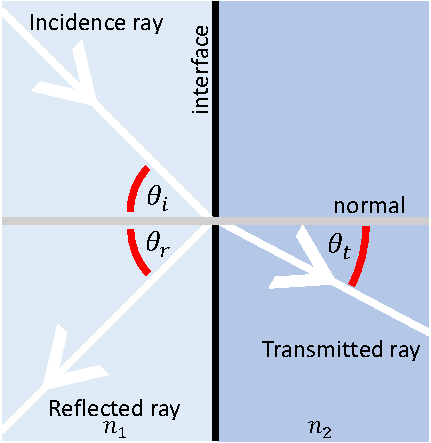
\includegraphics[width=0.4\linewidth]{figures/interface_fresnel_schematic.pdf}
  \caption{}
  \label{fig:fresnel_interface}
\end{figure}

Figure~\ref{fig:fresnel_equations} shows the phase change when reflecting off a silver mirror. At 45 degrees incidence angle there is a substantial difference between s and p-polarization, that becomes even larger at larger angles of incidence. And, more importantly, a difference in the slope. This means that a finite sized beam with a certain angular width will have different phase tilt aberration depending on the polarization state that enters the system. In literature this effect is called the Goos-Hanchen shift. In high-contrast imaging systems such effects create beam-shifts that limit the coronagraphic performance \citep{Schmid18, millar2022polarization}.

Polarization aberrations can be estimated using polarization ray tracing where the Fresnel equations are applied for every surface that is encountered during the raytrace \citep{ashcraft2023poke}. A convenient way to represent the aberrations is in the Jones pupil format. The Jones matrix is determined for each pixel in the pupil, which means that we end up with four pupil images ('xx', 'xy', 'yx' and 'yy'). The Jones pupil can then be used in high-contrast imaging physical optics simulations to estimate the interaction of the polarization aberrations with coronagraphs \citep{Anche23} or adaptive optics residuals \citep{millar2022polarization}. Recent simulations suggest that polarization aberrations could impact the extremely large telescopes at 1 to 3 \ld{} \citep{Anche23}. However, the strongest effects are seen in space-based coronagraphic systems that require a deep raw contrast of $10^{-10}$ to $10^{-8}$. Current systems typically encounter polarization aberrations at the $10^{-8}$ level \citep{mawet2011recent, seo2019testbed, baudoz2024polarization}. Common strategies are to put the whole instrument between polarizers to ensure only one polarization state is propagated. This ensures that the aberrations are controllable. However, this approach loses 50\% of the light. Current research is focused on finding solutions to mitigate the effects, either by optimizing coatings of the optics \citep{balasubramanian2005polarization,miller2022birefringent}, or by active wavefront control \citep{mendillo2021dual} and by improving the polarization leakage of the coronagraph \citep{Doelman20, Doelman23}.

\section{Focal plane wavefront sensing}

Imperfections in the manufacture of the optics within a high contrast instrument and the changing environmental conditions result in speckles in the final \ac{scfp}.
%
Several techniques for optical sensing of these residual aberrations using telemetry or metrology within the instrument have been partially successful in sensing and removing these aberrations with closed loops, using actively deformable optics to provide correction for the sensed modes.
%
Ultimately, these methods cannot sense the time-varying aberrations within the last optical elements before the \ac{scfp}, and so several methods have been developed to measure and characterise optical aberrations using the images from the \ac{scfp}.
%
The fundamental challenge is that the vast majority of the science focal plane detectors are photodetectors, and so they do not record the complex amplitude of the incoming electric field in the wavefront, but record only the intensity.

% ITERATIVE and FAST AND FURIOUS
The result is that an intensity image of the \ac{psf} cannot be uniquely inverted to give the phase and amplitude of the wavefront in the pupil of the system: an arbitrary wavefront can be represented as the weighted sum of a series of even $f(r)=-f(r)$ and odd $f(r)=-f(-r)$ point symmetric functions.
%
Odd functions produce \acp{psf} with point symmetry (e.g. tip/tilt, coma) but even functions produce the same \ac{psf} with the same amplitude but opposite sign - consider a wavefront with focus, which has $\psi(r) = a\sqrt{3}(2r^2-1)$, and both $a$ and $-a$ will result in the same intensity distribution in the focal plane.
%
One of the earliest methods for phase retrieval is therefore an iterative method, the Gerchberg-Saxton algorithm \citep{Gerchberg72}.
%
In this method, an estimate of the \ac{pp} phase is made by inverse Fourier transforming the \ac{psf} and applying the (incorrect) recovered phase in the \ac{pp} via a \ac{dm} or some other active optic.
%
The resultant science camera \ac{psf} will be closer to the ideal \ac{psf}, and so this loop is repeated until it converges to a flat wavefront - this can be a time consuming process requiring many iterations to get to the required precision.
%
A more rapid optimisation can be made by making informed guesses on the applied phase aberrations \citep{Gonsalves02}, and one such method is the ``fast and furious'' algorithm \citep{Keller12} that has been verified in lab \citep{Wilby18} demonstrated on-sky \citep{Bos20} on the SCExAO system. 

% DIVERSITY AND EFC METHODS
In order to measure the complex amplitude of the \ac{psf} without an iterative process, a diversity has to be introduced into the focal plane image, either temporally or spatially \citep[see ][ for a review of these]{Fienup13,Gonsalves14}.
%
For a single point source, all the light in the focal plane is coherent with respect to the core of the \ac{psf}.
%
A deformable element within the instrument can then introduce phase shifts into the pupil image that then change the resultant complex amplitude for each location in the focal plane of the science camera.
%
Each pixel in the focal plane then becomes an intensity interferometer, and if four phase shifts that reasonably sample between $0$ and $2\pi$ radians are introduced into the instrument, then the four recorded \ac{psf} intensity images can be fit to give an estimate of the complex amplitude at each location in the focal plane.

Calculating the appropriate phases that will result in an optimal sampling and estimate of the complex amplitude for HCI algorithms was presented with a unified formalism by \citet{Giveon09,Giveon10}, called Electric Field Conjugation (EFC).
%
In these papers it was shown that two pairs of complementary \ac{dm}actuations can provide enough phase diversity to measure the complex amplitude across the focal plane out to the spatial sampling of the mirror actuators.

%Methods include using separate regions of the focal plane to act as proxies for the behaviour of aberrations within the scientifically relevant field of view.
%
%This was tried by Wilby with (REF REF), 

One \ac{dm} enables correction of phase only aberrations in the science camera \ac{psf}.
%
If the aberrations include amplitude as well as phase, then correction with one \ac{dm} will result in one side of the \ac{psf} becming dark, but the other side will not.
%
This is solved with two \acp{dm} (with one \ac{dm} between a focal and \ac{pp} to allow for both amplitude and phase control) which can act in tandem to correct both amplitude and phase aberrations and correct a 360 degree region in the field of view.
%

\todo{mention a paper with the theory of this, then lab and on-sky demonstrations of this.}


%Estimating at the \ac{scfp} removes the NCPA entirely, but it is dependent on the robustness and sensitivity of the estimation method.
%
The \acl{scc} \citep[\acs{scc}; ][]{Baudoz06} principle takes light from the telescope, splits it into two beams, filter one beam through a pinhole and recombine the two beams in a Fizeau configuration in the \ac{scfp}.
%
All the speckles in the focal plane are subsequently modulated by a set of cosine fringes, the relative position of the fringes encoding the complex amplitude of the electric field of the \ac{psf}.
%
Any exoplanets or other point sources emit photons that are incoherent with the speckles, and so fringes do not appear at the location of the planet.
%
Simulations demonstrate \citep{Galicher10} bandwidths of up to 5\% and contrasts possible down to $10^{-10}$.

A modification on the \ac{scc} principle uses a modified \ac{fpm} to send more light to the pinhole used to generate fringes in the \ac{scfp}.
%
Adding a ramp of phase with a small amount of power in the \ac{fpm} within 3 \ld{} generates a spot of light that is offset from the pupil image in the PP.
%
This enables shorter exposures to capture the speckles in the \ac{scfp} and provide correction, called the \acl{fast} \citep[\acs{fast}; ][]{Gerard18} with laboratory measurements demonstrating $3\times 10^{-4}$ contrast \citep{Gerard22}.
%
Additional spectral modulation increases the throughput to produce the \acl{smscc} \citep[\acs{smscc}; ][]{Haffert22a}.

\begin{armarginnote}[]
  \entry{SCC}{Self Coherent Camera}
  \entry{FAST}{Fast Atmospheric SCC}
  \entry{SM-SCC}{Spectrally Modulated SCC}
\end{armarginnote}

% PSI
A closed loop AO system leaves time-varying wavefront aberrations propagating through to the \ac{scfp}.
%
Short exposure images freeze these speckles and show that for a given location in the \ac{scfp} the flux changes as a function of time.
%
For thermal infrared science cameras on ground based telescopes, the science images saturate rapidly due to the thermal background of the Earth's atmosphere, and so the rapidly changing speckles naturally provide a ``free'' source of phase diversity.
%
Under the assumption that the \ac{ncpa} is changing on a much slower timescale than the speckles generated by the wind driven halo, the \ac{wfs} can provide an estimate of the complex amplitude of the \ac{scfp}, plus a fixed \ac{ncpa} term.
%
Phase Sorting Interferometry \citep[PSI; ][]{Codona13} enables a virtual interferometer to be constructed for each location in the \ac{scfp}, and the \ac{ncpa} calculated.
%
This was successfully demonstrated as a post-processing technique at thermal infrared wavelengths at the MMT Observatory with the Clio camera.

Electric Field Conjugation has been tested on the internal sources of \ac{sphere} (a contrast of $5\times 10^{-7}$ at 150 mas from the optical axis in a few minutes using the \ac{sphere} instrument).
%
This was demonstrated on-sky with the \ac{aplc} coronagraph and \ac{sphere} \citep{Potier20,Potier22}, using an iterative scheme to clear a dark hole on one side of the science camera \ac{psf}, and with the \ac{fqpm} coronagraph in \ac{sphere} \citep{Galicher24}.

XXXX

coronagraphic phase diversity
COFFEE jean-francois sauvage 2012 \citep{Sauvage12}.

\begin{figure}[ht]
  \centering
  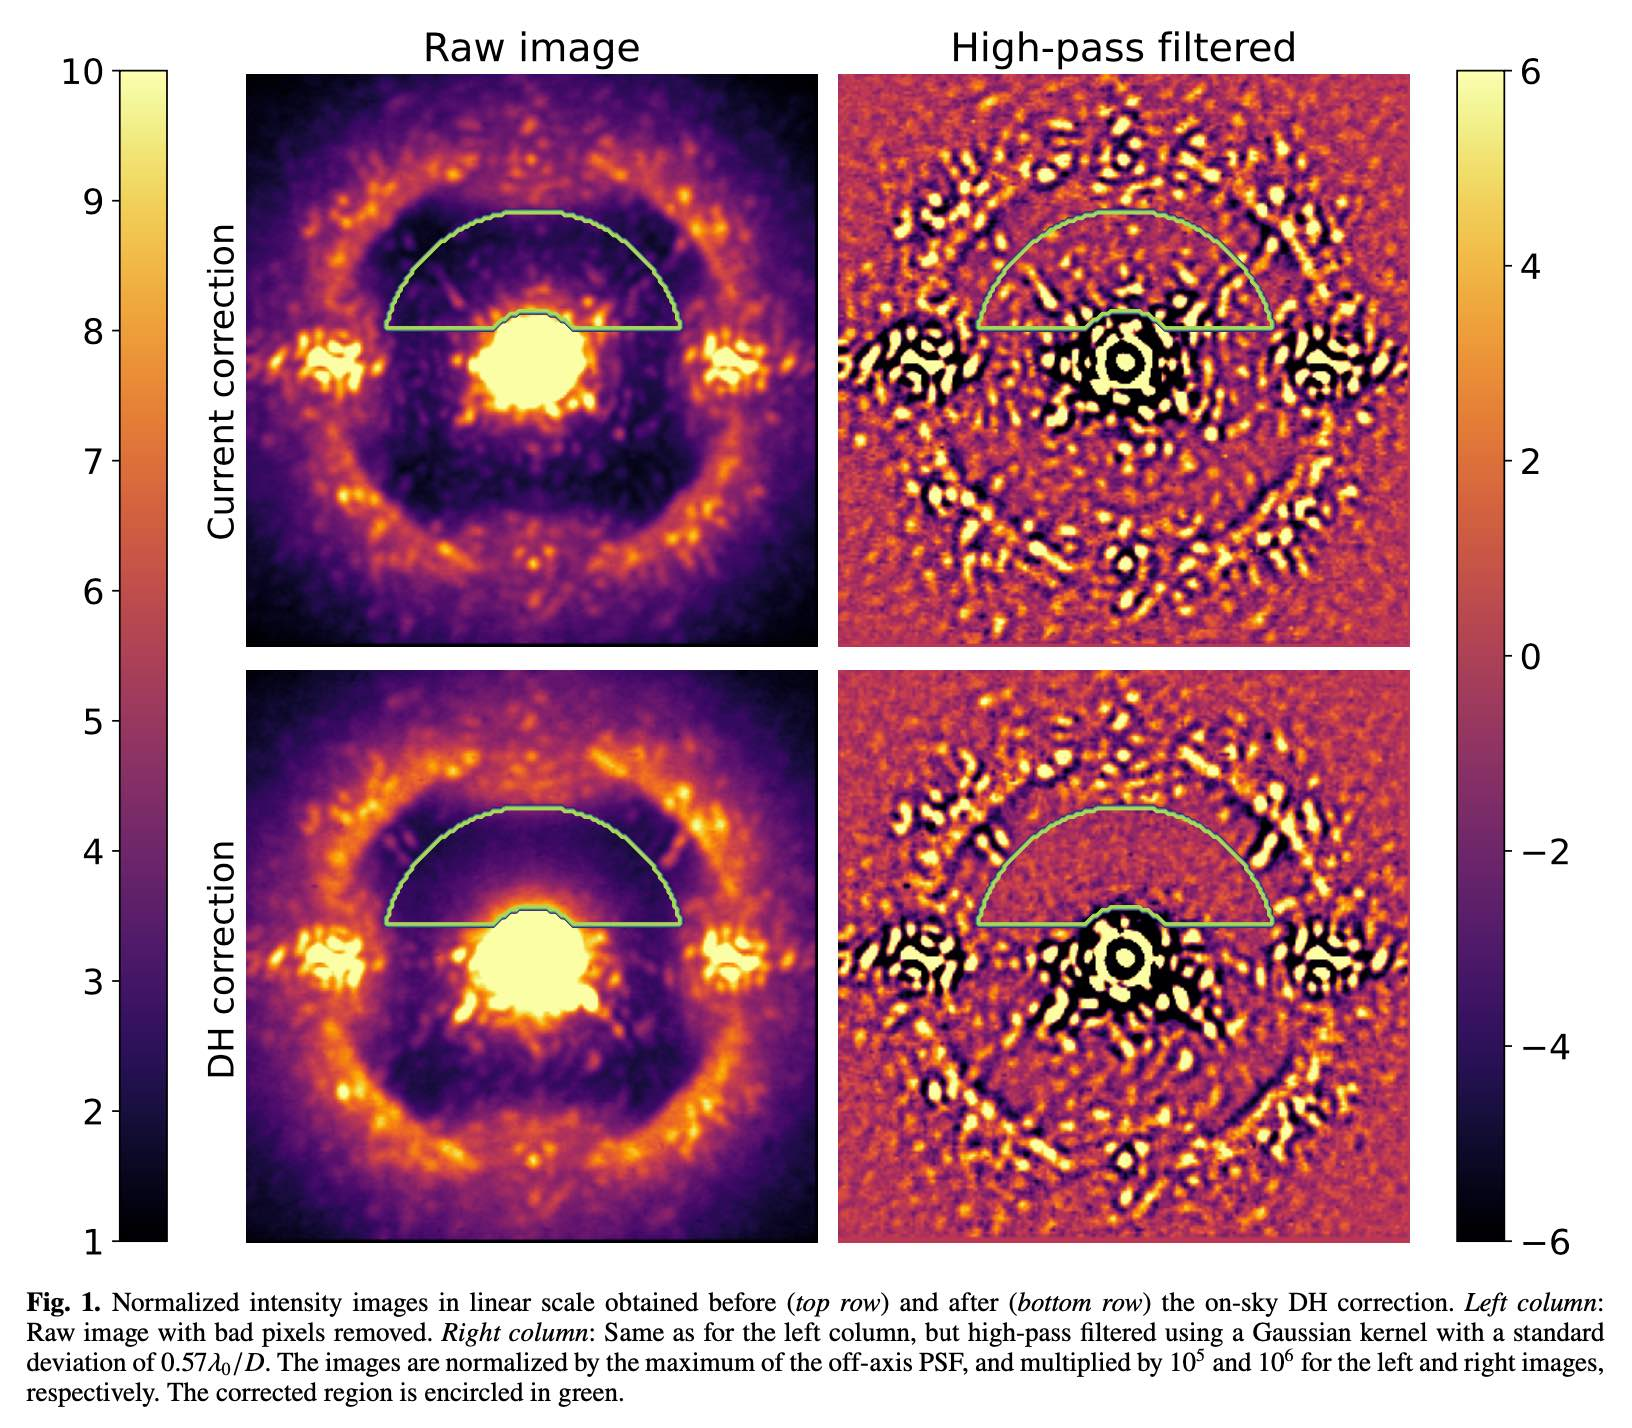
\includegraphics[width=0.6\linewidth]{figures/potier2022.jpg}
  \caption{}
  \label{fig:fpwfsclean}
\end{figure}

\notebooksuggestion{SH: get this from HCIpy Simple dark hole generation with predefined shapes - can use the new autodiff approach.}

%\lipsum[2-4]


% \section{Coronagraphic wavefront sensing} REMOVE THIS AND MERGE WITH FPWFS SECTION 

% Ideally, the coronagraph and \ac{wfs} used to measure the electric field on the \ac{scfp} are integrated together in the design of the instrument.

\section{Rejected light wavefront sensing} 

Focal plane coronagraphs require the star to be aligned on a \ac{fpm} to a high degree of precision to prevent leakage of starlight into the \ac{scfp}.
%
Measuring the centroid of the star is not possible due to the insensitivity to low order aberrations of the coronagraphic \ac{psf} in the \ac{scfp}.
%
Low order aberrations can, however, be measured from the light reflected from the \ac{fpm}.
%
A design that uses a central opaque dot with a reflective annulus that takes light from 0.72 \ld{} to 1.2 \ld{} shows that this signal can keep tip tilt to around $10^{-3}$\ld{} for a baseline telescope and observation of a 6th magnitude star \citep[Coronagraphic low order \ac{wfs}; CLOWFS ][]{Guyon09}.
%
For coronagraphs that use a phase mask in the focal plane (such as a Vortex mask), another method is required.
%
By putting in a reflective Lyot stop, the rejected light is reimaged to a separate camera and this forms the error signal for low order aberration measurements and is called the Lyot-based Low Order \ac{wfs} \citep[LLOWFS; ][]{Singh14,Singh15}.
%
The LLOWFS can measure tip-tilt down to $\sim 10^{-2}$\ld{} (equivalent to 2–12 nm at 1.6 \mum{}) per mode on the \ac{fqpm}, with on-sky results being somewhat larger \citep{Singh15}.
%
Both these methods deliberately introduce defocus into the rejected light image, so that the focus ambiguity is removed and tip-tilt and focus modes can be simultaneously measured.

\ac{zwfs} are FP masks that have a $\pi/2$ phase shifted dimple with a diameter of 1-2\ld{}.
%
The resultant pupil image intensity distribution encodes the phase of the wavefront.
%
The segmented geometry of the space telescope HabEx and LUVOIR concepts require picometer measurements that are fed into the control loop for the \ac{dm} in the coronagraph - this was demonstrated for low and mid spatial frequencies with a \ac{zwfs} up to the \ac{dm} control radius in \citet{Ruane20}.


A modification of the Hybrid Lyot Coronagraph (HLC) uses a Dual Purpose Mask for the \ac{fpm}, making a Dual Purpose Lyot coronagraph (DPLC).
%
This DPM is a tiered metallic focal plane occultor suppresses starlight in the transmitted coronagraph channel and a dichroic-coated substrate to reflect out-of-band light to a wavefront sensing camera.
%
It acts as a \ac{zwfs} in reflection, sending out-of-band light to a CLOWFS to maintain high contrast in the science focal plane \citep{Ruane23}.

XXXX

%
By putting a \ac{zwfs} at the location of the \ac{fpm} in a PIAA coronagraph, this can approach fundamental sensitivity limits within the instrument \citep{Haffert23}.


Low-order wavefront control using a Zernike sensor through Lyot coronagraphs for exoplanet imaging
\citep{Pourcelot22,Pourcelot23} NOTE that this has reject light passingt hrough and the science camera light is reflected! Unusual geometry due to lab setup.

cite Por 2023 presentation on the SPIE website or 2021 SPIE \ac{zwfs} and \ac{aplc} integrated. 


HiCAT dark zone demonstration \citep{Soummer22} is where ALL these things are combined. 


\section{Summary of new high contrast instruments}

MAK suggestion: we make this a table instead.



%MagAOX paper.... Mcleod et al. 2023
GMagAOX from Jared Males 2022/2024 \citep{Males22}.

ADD GMAgAO-X in design review.
SPHERE+
GPI 2.0


Second generation instruments are already in development for HCI of terrestrial worlds: ELT's PCS \citep{Kasper21} and TMT's PSI \citep{Jensen-Clem22,Fitzgerald22} and these factors are already being considered in their optical and system level designs.


XXX ANDES (high dispersion spectro) has a tiny IFU (HARPS verion for ELT)



Visible extreme AO on \acp{elt} for Prox b: \citep{Fowler23}


\section{Photonic versus bulk optics}

Optics change the complex amplitudes of wavefronts as they propagate through coronagraphs.
%
Classical optics (referred to as `bulk optics') are typically many thousands of times larger than the wavelength of light they shape and require precise and stable optomechanical components to accurately modify these wavefronts.
%
Integrated (or `photonic') optics enable direct manipulation of the complex electric fields at the scale of the wavelengths used.
%
Miniaturisation of previously discrete macro optics and their manufacture within a single homogeneous substrate removes both the requirement for separate optomechanical alignment and temperature related misalignment that is associated with their mechanical mounts.
%

Beam combiners that are required for optical and NIR interferometers require temperature and vibration controlled optical tables with sub-wavelength stability tolerances and alignment for the beamsplitters and associated optics.
%
Manufacture of waveguides within optical materials that perform the beam division and combination considerably simplify the optomechanical requirements, but then the challenges are in coupling the light from the macro optics into the substrates whilst keeping the transmitted efficiency high: diffraction limited optics are required to form \acp{psf} that couple efficiently into the near-single mode sized microoptics.
%
Early examples include beam combiners for optical astronomical interferometers \citep[for example the IOTA/IONIC beam combiner; ][]{Berger01} and photonic lanterns, see \citet{Leon-Saval10} and references therein.
%
Typical coupling efficiencies are on the order of 10\%, increasing to 90\% for more recent designs, for example the efficient injection from large telescopes into single-mode fibres \citep{Jovanovic17}.
%
Full electromagnetic propagation is required to design and evaluate these photonic systems, but their complexity also enables new optical designs which can be combined to form compact, robust instrumentation, see the reviews in \citet{Minardi21,Jovanovic23}.
%
Photonic devices that are relevant for high contrast imaging applications include:

{\bf Photonic Lanterns: } Coupling multi-mode light into monomode photonics is done using photonic lanterns, a multimode input converted into the areal equivalent of a number of single mode optical channels, \citep{Norris22}.

{\bf Closed Ring Resonators: } A device equivalent to Fabry-Perot etalons can be constructed by etching an elongated loop with one half of the loop parallel to the waveguide - frustrated transmission between the waveguide and the closed loop is modulated as a function of the number of integer wavelengths around the closed loop (REF REF REF).

{\bf Bragg gratings: } than enable modulation of diffraction \citep{FaggingerAuer24}.

All these photonic concepts are being considered for the design of coronagraphs for next generation space telescopes in order to image and characterise exoplanets, exploring concepts of different combinations of photonic and bulk optics \citep{Desai23a}.

%Photonic devices that combine several aspects of these modules include PIMMS: a photonic integrated multimode microspectrograph from \citet{Bland-Hawthorn10}.
%
%Focal Plane Wavefront Sensing with Photonic Lanterns are demonstrated in \citep{Lin20} and their theory \citep{Lin22}, nulling with a mode selective photonic lantern \citep{Xin22}.


%Advances in industry and the requirement for increasingly complex and denser signal transmission lines from the telecommunications industries have made more complex designs realisable for astronomical optics.
%
%The optical designs are considerably more challenging, since geometrical optic limits are not a valid approximation.
%
 
%https://pure.uhi.ac.uk/en/publications/an-integrated-optics-3-way-beam-combiner-for-iota (REF) 

%% Emiel - presented at SPIE 2024 on integrated coronagraphs and photonics - NOTE ONLINE YET.


\section{Quantum optimal detection}

Quantum optical detection \citep{Lu18} enables the distinction between two incoherent point sources within the classical Rayleigh diffraction limit.
%
This can be done by a specific linear optic reformatting of the wavefront followed by a photon counting detector.
%
More specifically, for exoplanet detection where the separation is smaller than the diffraction limit and the flux ratio much smaller than 1 \ld{}, for thermalised incoherent sources (e.g. a star and a planet) you test for photons not being distributed in a point symmetric way \citep[e.g. ][]{Huang21}.
%
\citet{Desai23} derive these limits in Achieving Quantum Limits of Exoplanet Detection and Localization.

\section{Algorithms for estimating the instantaneous PSF}

\notebooksuggestion{KLIP with removing varying number of modes and annular rings.}

Deviations from the ideal optical prescription of telescope and instrument optics result in wavefront errors which manifest themselves as intensity deviations from the theoretical \ac{psf}.
%
Furthermore, these deviations change in intensity and position with time in the \ac{scfp}, and these can be equal to or larger than the flux from the astrophysical object next to the star.
%
The question is then how to estimate the science camera \ac{psf} for every single science camera exposure  and subtract this estimate from the science camera image leaving only the flux from astrophysical objects adjacent to the target star.
%
This becomes more complicated when the position and brightness of the exoplanet is not known.
%
%The flux from the stellar halo and the flux from the exoplanet are generated from different processes: the stellar halo is generated from wavefront distortions in the telescope and instrument optics and through diffraction, meaning that the halo is coherent with the central star.
%
Several diversities - properties of the exoplanet that are not the same as the stellar halo - can differentiate between them.
%
The most important of these are:

\begin{itemize}
    \item Angular diversity: For an alt/az telescope, the planet has a predictable angular position and velocity with respect to the orientation of the instrument optics.
    \item Spectral diversity: The planet has a different spectral energy distribution, meaning that the relative flux between star and planet changes with wavelength.
    \item Polarimetric diversity: The light from star is almost completely unpolarized, but reflected light from clouds or dust around the exoplanet become polarsied under single scattering \citep{Gledhill91}.
    \item Wavelength diversity: The stellar halo scales with \ld{}, but the planet remains at the same linear separation on the sky.
    \item Coherence diversity: The exoplanet flux is not coherent with the stellar halo and so does not interfere with it.
    \item Stochastic Speckle Discrimination: and the intensity fluctuations of the Airy core on ground based telescopes has a different statistical distribution \citep{Gladysz09}.
\end{itemize}

Many algorithms have been developed to take one or more of these diversities and provide estimates of the science camera \ac{psf}, using different linear combinations of the science camera images to estimate the instantaneous science camera \ac{psf}.
%
%These ability of these algorithms to recover the exoplanet flux varies with the separation between the star and planet, the total amount of angular rotation seen on sky, and 
{\it Hubble Space Telescope} (HST) images of circumstellar material showed residual speckles that obscure the faint circumstellar environment, even after the subtraction of an image of a nearby star used as a reference \ac{psf}.
%
The concept of ``roll subtraction''  \citep{Schneider98} was used to estimate and remove these residual speckles.
%
Two or more images of the science target were taken with the telescope set at different angles about the target axis, so that the astronomical field would be rotated with respect to the (almost static) speckle field.
%
This was demonstrated in \citet{Schneider99} with the image of the disk around HR~4796A.
%
Even with the HST, the roll observations were taken within 25 minutes of each other to minimise changes in the telescope's optical path resulting from the ``breathing'' of the telescope optical assembly as it passed from day to night in its low earth orbit \citep{Bely93}.

With a ground based telescope, the speckle field changes on shorter timescales and with increased complexity because of (i) a continuously changing gravity vector on the telescope and instrument (ii) temperature and mechanical variations in the optomechanics within the instrument and (iii) changes in the performance of the adaptive optics system due to changing atmospheric conditions.
%
Angular Differential Imaging \citep[ADI; ][]{Marois06} has become a fundamental algorithm for many ground based telescope observations where significant sky rotation occurs during the observations of the planet.

Exploiting narrow band absorption features in the gas giant exoplanet spectrum enabled Methane Spectral Imaging (MSI), with TRIDENT \citep{Marois05} being one of the first cameras built to exploit this, along with the SDI camera at the MMT and VLT \citep{Biller07-1}.
%
With AO systems reaching to optical wavelengths, this has had a renaissance with Hydrogen alpha imaging with the MUSE integral field spectrograph and the discovery of the accreting protoplanet PDS~70c \citep{Haffert19}.

Estimating the stellar halo with images at nearby wavelengths was generalised with the use of integral field spectrographs, where many science camera \acp{psf} are sampled at different wavelengths simultaneously to form $(x,y,\lambda)$ data cubes.
%
Resampling the image slices into the same \ld{} spatial scale radially smears out any exoplanet signal, so subtracting off a median of these images removes the stellar halo but keeps most of the planet flux intact, making it visible when the median subtracted cube is resampled into the sky coordinates and combined to produce the \ac{psf} subtracted image, generalised as Spectral Differential Imaging \cite[SDI; ][]{Sparks02} and demonstrated on-sky with SINFONI \citep{Thatte07}.

For higher spectral resolutions, the spectrum of the exoplanet begins to resolve the individual rotational-vibrational transitions, enabling High Spectral Contrast Imaging \citep[including the detection of HD~209458b ][]{Snellen10} and then generalising into the principle of molecule mapping in directly imaged exoplanets such as Beta~Pictoris~b \citep{Hoeijmakers18}.

Stochastic Speckle Discriminaton \citep[SSD; ][]{Gladysz09} is possible using short exposure images with the Airy core unsaturated.
%
Photon counting devices enable this detection method to work - this was demonstrated using an MKIDS detector and has led to the discovery of a substellar companion using this technique \citep{Steiger21} and also on extended sources such as circumstellar disks \citep{Steiger22}.

%Coherence Differential Imaging: with MKIDS and Ben Mazin VAMPIRES, done it on SPHERE.

\todo{Figure: show example of post processing. pick favourite image from a paper!}

\section{Conclusions}

Since the first detection of planets outside our solar system with the pulsar planets \citep{Wolszczan92} using pulsar timing, and the first exoplanet around a solar-type star \citep[51 Peg b; ][]{Mayor95} using radial velocity measurements on the star, we now have thousands of planets indirectly detected with radial velocity and transit methods.
%
Direct imaging of exoplanets have revealed dozens of young, self-luminous gas giant planets \citep{Currie23,Chauvin24} and with the minimized infrared background accessible with the \ac{jwst}, we are entering the era of directly detecting sub-Jupiter mass planets.

\acp{elt} with extreme AO systems and the next generation of space telescopes enable the reflected light detection of planets around the nearest stars.
%
The direct imaging of exoplanets is a dynamic and rapidly changing field, with each decade of suppression bringing new challenges and researchers searching for and finding solutions to them.
%
We have the coronagraphs in theory, verified in the laboratory, and demonstrated on sky.
%
We find technical solutions and develop algorithms to tease out these faint signals against the almost overwhelming glare of their parent stars.

It is perhaps inevitable that in the next decade we will be imaging and characterising pale blue dots around our nearest neighbours, and we will take one further step to seeing if the Earth is truly unique.

%Disclosure
\section*{DISCLOSURE STATEMENT}
The authors are not aware of any affiliations, memberships, funding, or financial holdings that
might be perceived as affecting the objectivity of this review.

% Acknowledgements
\section*{ACKNOWLEDGMENTS}
M.\ A.\ K.\ acknowledges useful conversations with
Phil Hinz, Andrew Skemer at the Humblesea Brewing Company.

To achieve the scientific results presented in this article we made use of the \emph{Python} programming language\footnote{Python Software Foundation, \url{https://www.python.org/}}, especially the \emph{SciPy} \citep{virtanen2020}, \emph{NumPy} \citep{numpy}, \emph{Matplotlib} \citep{Matplotlib}, \emph{emcee} \citep{foreman-mackey2013}, and \emph{astropy} \citep{astropy_1,astropy_2} packages.
%
The HCI simulations were calculated with \emph{HCIpy} \citep{Por18}.
%
This Article is reproducible using the \emph{showyourwork!} workflow management tool \citep{Luger2021}.
%
This research has made use of NASA's Astrophysics Data System Bibliographic Services.

This document contains \total{citnum}\ references.

% References

\bibliographystyle{ar-style2}
\bibliography{bib}

\section*{RELATED RESOURCES}

This manuscript was prepared using the \project{showyourwork} package\footnote{\url{https://show-your.work}} and the source code used to generate each figure is available in a public \project{GitHub} repository\footnote{\url{https://github.com/mkenworthy/ARAA_HCI}}.

\end{document}
